\section{Backgrounds}

An accurate description of the background process is an essential aspect of any analysis since it affects the extraction of signal yields.
The main background sources differ between the three channels, but generally belong to the category of \textit{reducible background}.
This class contains processes which have a different final state from the signal.
However, either due to additional particles produced in combination which may produce a different signature in the detector,
other collisions in the same bunch crossing (pileup),
or other errors in the reconstruction procedure,
they produce events which may erroneously pass the selection.
Often these backgrounds prove difficult to model in simulation,
and it becomes advisable to use a data-driven method for their estimation.

The other category comprises \textit{irreducible backgrounds},
which are processes that generate a final state with the same particles as the signal,
although the kinematic distributions may be different.
Usually processes in this class are estimated with simulation,
but in some cases it is possible to constrain their normalisation in a control region.

%% \subsection{Four lepton channel}
For the 4\Pl channel the predominant background component is the production of two on-shell \PZ bosons
and a photon that is either radiated as FSR from one of the leptons
or from a misreconstructed jet.
As described in Section \ref{sec:simulation}, it can be either produced from two quarks,
or proceed from a gluon initiated loop.
Additional backgrounds such as $\PQt\PAQt\PZ$ and VVV (V = \PZ, \PW) result in very small contributions.

%% \subsection{Three lepton channel}
In the 3\Pl channel the main background contributions are Drell-Yan + jets, $\PZ\PGg$ + jets
and $\PW\PZ$ plus a photon that is either radiated as FSR from one of the leptons or from a misreconstructed jet.
Another significant contribution comes from $\PZ\PZ \to 4\Pl$ where one of the leptons is lost or misreconstructed as a photon.
There is also a small fraction of events from $\PZ\PZ\PGg$ in which one of the leptons is outside the detector acceptance. \todo{should check in MC}
Additional backgrounds from rare processes such as $\PQt\PAQt\PZ$ and VVV (V = \PZ, \PW) result in very small contributions and are estimated with simulation.

\paragraph{Reducible background\\}
This group of backgrounds arises from processes in which some of the reconstructed leptons or photons do not correspond to real, prompt leptons from the vector bosons decay or photons from the hard process.
This particles can either be \nonprompt leptons or photons, or misidentified light-flavour jets.

\Nonprompt leptons come mainly from decays of heavy flavour mesons and electrons from asymmetric photons conversions,
while \nonprompt photons originate primarily from decays of light neutral mesons like \PGpz or \PGh.
Both leptons and photons in this category tend to be non-isolated from the nearby jet activity.

The other class is comprised of misidentified jets, mostly from light-flavour quarks, which can erroneously be reconstructed as either leptons,
if a track is associated to the main energy deposits, or as photons otherwise.
These misidentified photons tend to have a different energy distribution in the ECAL with respect to real photons,
which makes shower shape variables effective in separating this background from real photons.

In the following the terms \textit{fake leptons} and \textit{fake photons} are used to refer to both \nonprompt and misidentified objects.

\todo{Look in Wgamma or some other analysis more detail about nonprompt/misidentified photons}

\subsection{Fake Leptons}
To estimate the expected fake lepton background yield in the signal region,
dedicated control regions are defined with requirements similar to the signal region but in such a way not to contain signal events.
To enhance the \nonprompt lepton component, events in these regions are required to
have a number of leptons that fail the tight selection, while passing the loose criteria.
The other selections are identical to maintain similarity with the signal region.

The fake lepton background yield in the signal region is extrapolated from these regions
according to the probability for loose lepton candidates to pass also the final selection criteria (defined in Section 4.1.2).
These probabilities, referred to as fake rates, are estimated independently as illustrated in the following section.

\paragraph{Four lepton channel\\}
For the 4\Pl channel, two control regions are defined.
The former, named CR3P1F, one of the leptons of the $\PZ_2$ must fail the tight selection,
while the other three (2 from $\PZ_1$ and the other from $\PZ_2$) must pass the tight identification and isolation criteria.
It is expected to be populated by $\PW\PZ$, with contributions from Drell-Yan and $\PZ\PGg$,
along with a fraction of events from $(\PQq\PAQq/\Pg\Pg) \to \PZ\PZ$ where one of the prompt leptons fails the selection.

In the latter region, named CR2P2F, both leptons from the $\PZ_2$ fail the tight selection, while the leptons of the $\PZ_1$ pass the tight criteria.
This region is populated primarily by Drell-Yan events, with contributions from $\PZ\PGg$ and $\PQt\PAQt+X$.

This method was used by several analyses targeting a final state with four leptons from $\PZ\PZ$ decay~\cite{CMS-SMP-16-001, CMS-SMP-17-006, CMS-SMP-20-001, CMS-PAS-SMP-22-001},
and is described in detail in Reference~\cite{CMS-HIG-13-002} as the ``Method using opposite-sign (OS) leptons''.

\paragraph{Three lepton channel\\}
\note{At the moment, the data-driven fake estimate does NOT work in SR3P. Maybe we shouldn't discuss it if we don't use it.}

\note{SMP-16-002~\cite{SMP-16-002} (2015 data) uses a dijet region to measure the fake rate:
\textit{``The misidentification probability is measured from a sample of
dijet events enriched in nonprompt leptons. The sample is selected
with one jet passing the relaxed lepton identification requirements
matched to a single lepton trigger, defined as the probe lepton.''}}

\note{SMP-20-014~\cite{SMP-20-014} (full Run2) uses a L+j region:
\textit{``This CR is defined by requiring a single lepton with pT greater than 10 GeV, and at least
a reconstructed jet that is well separated from the lepton at $\DR(\PGg, j) > 0.7$. Contributions from
EWK processes are subtracted to obtain a pure nonprompt measurement region.''}}

\todo{Describe fake leptons method in 3L channel}

\subsubsection{Lepton fake rate measurement}
The measurement of the lepton fake rate, which is the probability that a fake lepton that passes the loose selection also passes the tight criteria,
is carried out in a separate control region which is enriched in contempt leptons.

This region, denoted as $\PZ+L$, is defined as containing a valid \PZ candidate whose leptons must have $\pt^{\Pl_{Z,1}} > 20 \GeV$ and $\pt^{\Pl_{Z,2}} > 10 \GeV$
and an additional lepton which passes the loose selection.
Additionally, the \PZ candidate must have a mass within 10 \GeV from the nominal peak,
and the missing energy must be $\MET < 20 \GeV$ to reduce the contribution from real leptons from $\PW\PZ$.
The last requirement means that this region is orthogonal to all of the regions in the 3\Pl channel, in which the MET is required to be greater than 30 \GeV.

The fake rate is measured on the third lepton in several bins of transverse momentum, separately for the barrel and endcap and flavour.
The measurement is done for each year of data taking, and the resulting rates can be seen in Figure \ref{fig:leptonFR}.

\begin{figure}
  \centering
  \subfigure [2016] {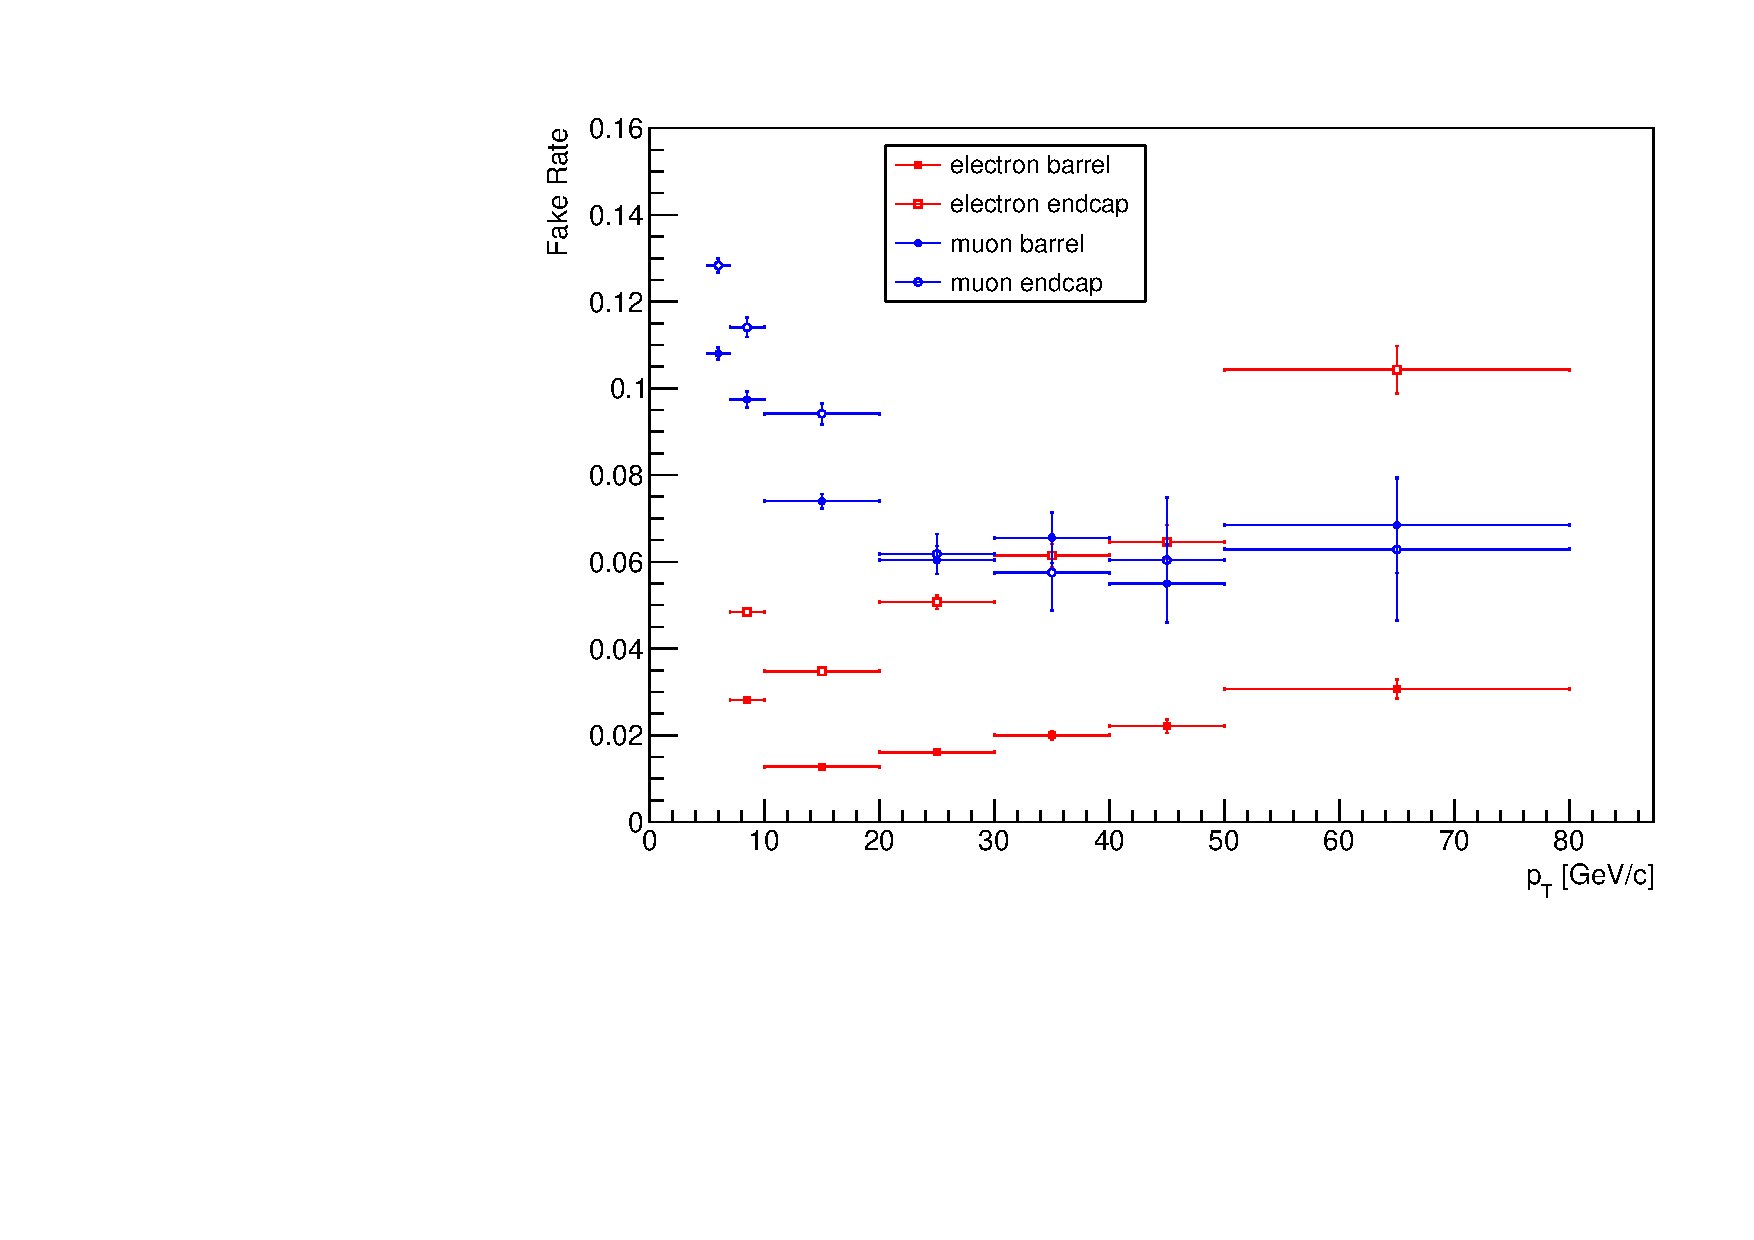
\includegraphics[width=.5\textwidth]{leptonFakeRate_2016.pdf}}%
  \subfigure [2017] {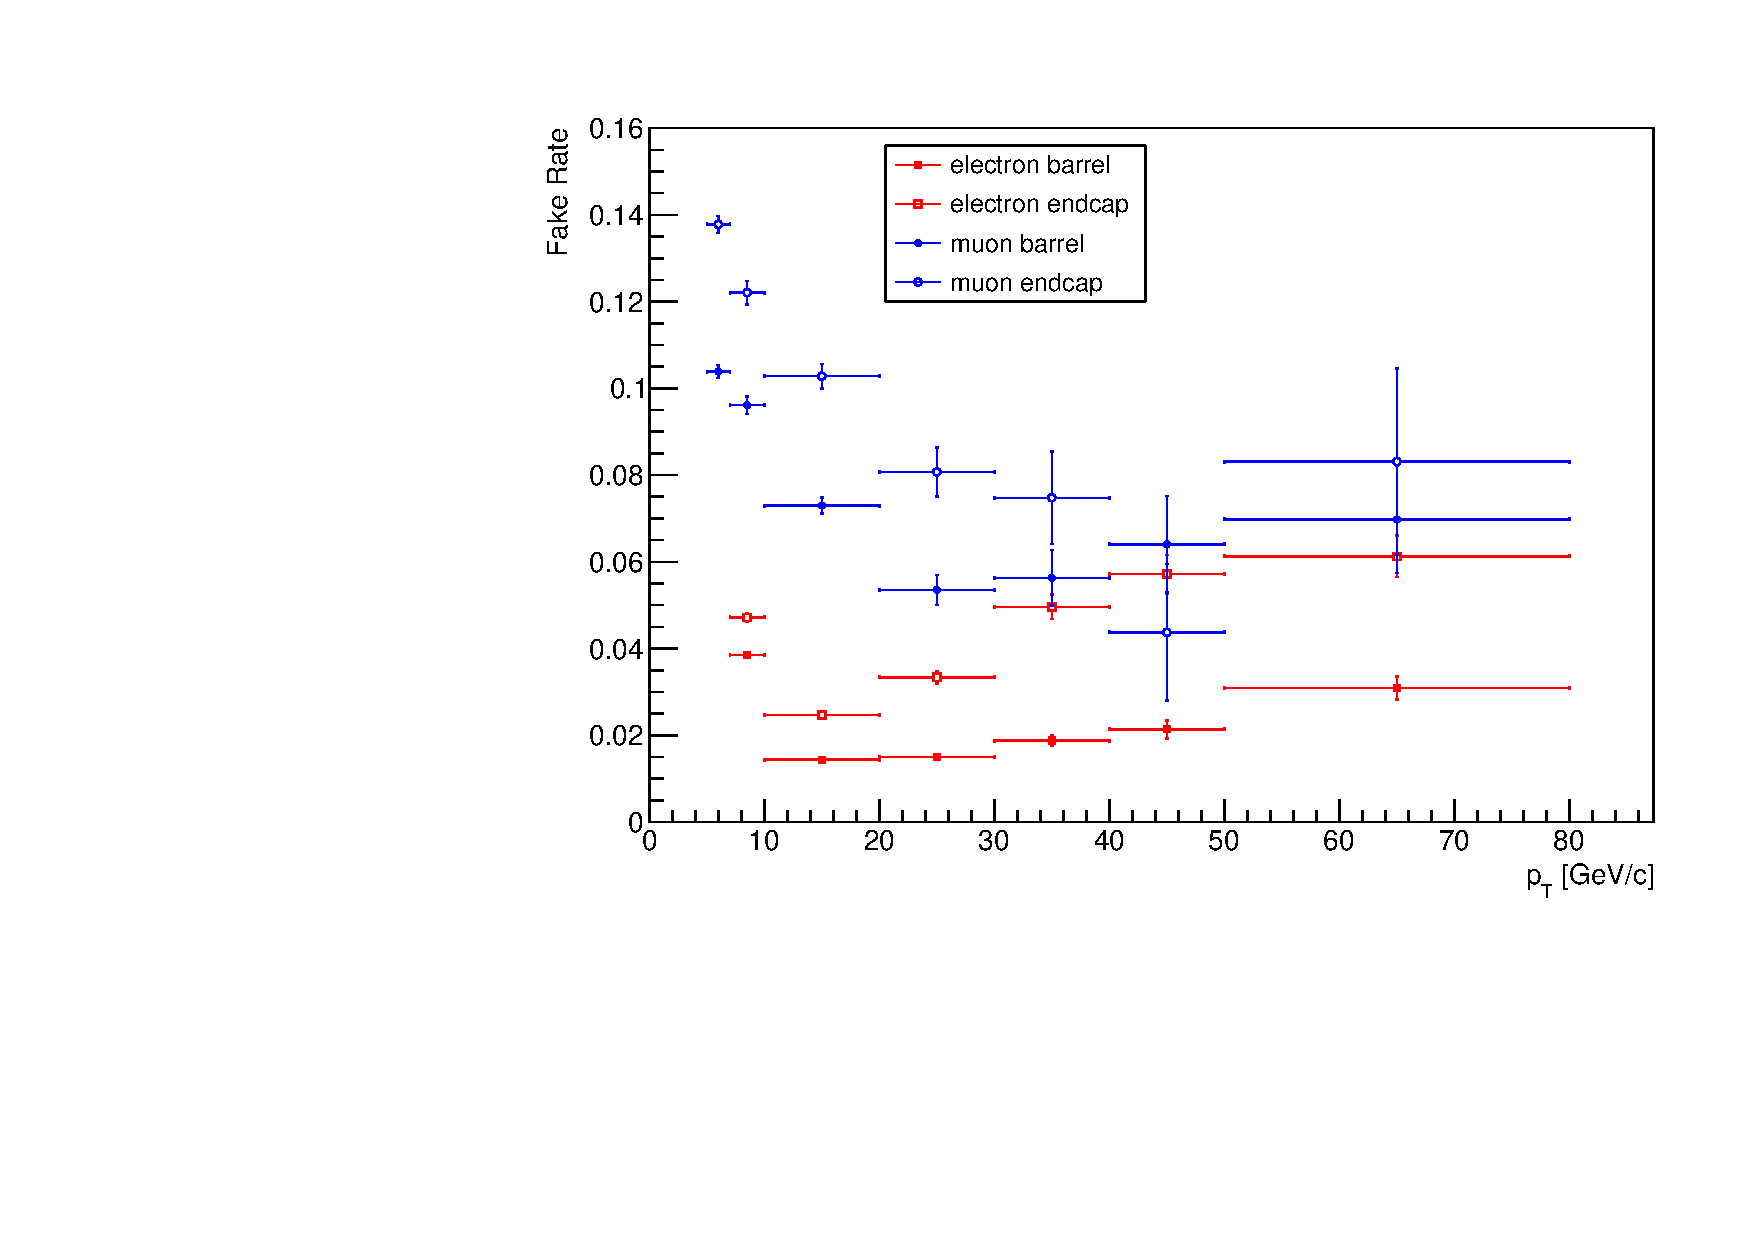
\includegraphics[width=.5\textwidth]{leptonFakeRate_2017.pdf}}\\
  \subfigure [2018] {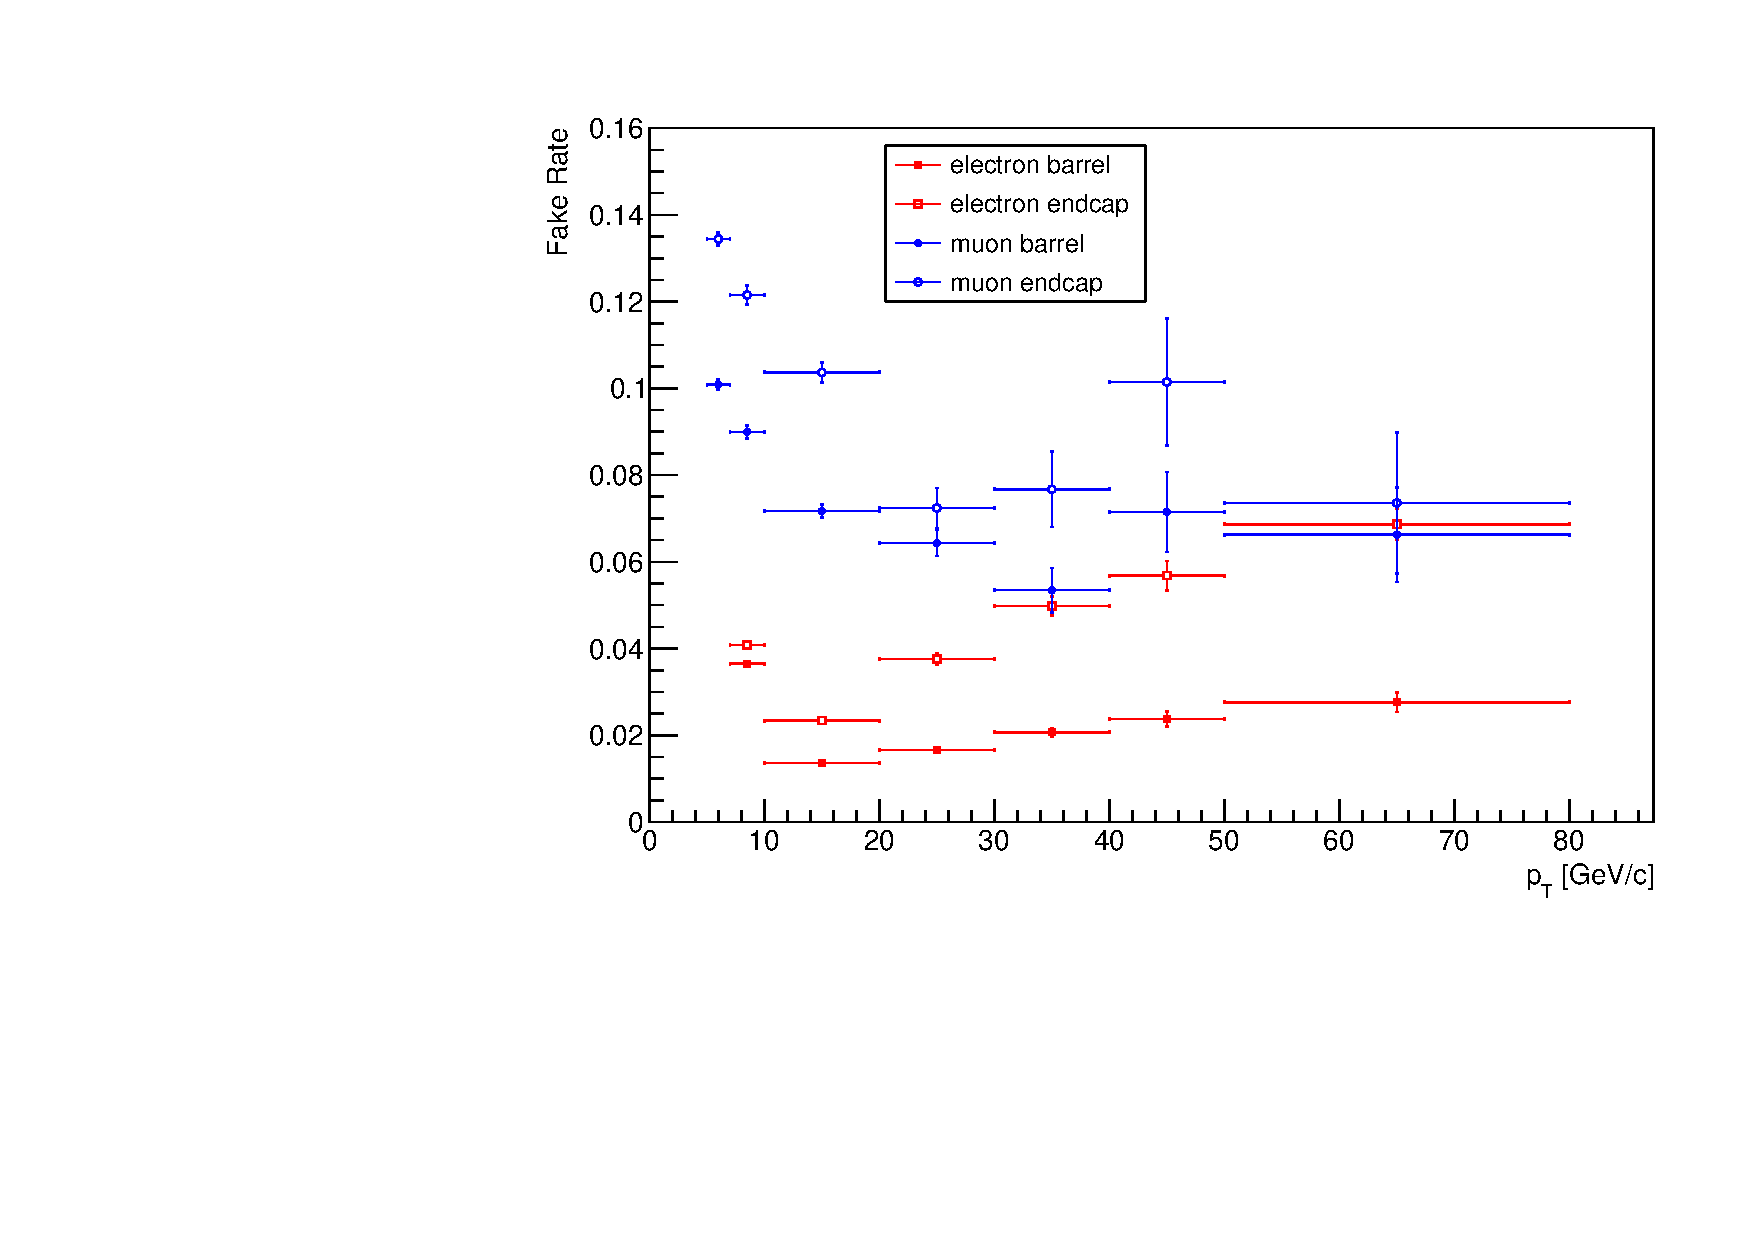
\includegraphics[width=.5\textwidth]{leptonFakeRate_2018.pdf}}
  \caption{Lepton fake rates measured in the $\PZ+L$ control region, for each year of data-taking.}
  \label{fig:leptonFR}
\end{figure}

The uncertainty on the fake lepton background estimation arises from the difference in composition of the
background processes in the region where the fake rate is measured and where it is applied.
This uncertainty was measured by several analyses \todo{cite} and found to be \todo{how much?}.

\subsubsection{Lepton fake rate application}
\paragraph{Four leptons channel\\}
Once the fake rates are estimated they are applied to the CR2P2F and CR3P1F dedicated control regions to estimate the fake lepton background yield in the 4\Pl signal region.

The expected reducible background in the signal region is given by the sum of two terms:
\begin{itemize}
  \item A 3P1F component, from events with on fake lepton, estimated from the CR3P1F region.
  \item A 2P2F component, from events with two fake leptons, estimated from the CR2P2F region.
\end{itemize}

The 3P1F and 2P2F components are given by the number of events in the respective regions, weighted by factors dependent on the fake rates:
\begin{subequations}
  \begin{align}
    \label{eq:lepFR_3P1Fto4P}
    N^{from\ 3P1F}_{SR} &= \sum_{i \ins 3P1F} \frac{f_a^i}{1-f_a^i}, \quad where\ a = 3, 4
    \\
    \label{eq:lepFR_2P2Fto4P}
    N^{from\ 2P2F}_{SR} &= \sum_{j \ins 2P2F} \frac{f_3^j}{1-f_3^j} \frac{f_4^j}{1-f_4^j}
  \end{align}
\end{subequations}
where $f_3^j$ and $f_4^j$ correspond to the fake rates of the two loose leptons in the j-th event.

However, the CR3P1F region itself has a contribution from fake lepton background events from the CR2P2F region.
These are events with two genuine leptons and two fakes, where only one of the fakes passes the tight selection, thus winding up in the CR3P1F region.
The expected number of background events in the CR3P1F region, $N^{from\ 2P2F}_{3P1F}$,
can be computed from the number of events observed in the CR2P2F control region, $N^{bkg}_{2P2F}$,
by weighting each event in the region with a factor dependent from the fake rates:
\begin{equation}
  \label{eq:lepFR_N3P1F}
  N^{from\ 2P2F}_{3P1F} = \sum_{i \ins 2P2F} \left( \frac{f_i}{1-f_i} + \frac{f_j}{1-f_j} \right)
\end{equation}

Summing all the contributions, one obtains for the signal region:
\begin{equation}
  \begin{split}
    \label{eq:lepFR_4P}
    N^{bkg}_{SR} &= \sum \frac{f^a_i}{1-f^a_i} \left( N_{3P1F} - N^{from\ 2P2F}_{3P1F} \right) + \sum_{j \ins 2P2F} \left( \frac{f_j}{1-f_j} \frac{f_j}{1-f_j} \right)
    \\
                 &= \sum_{i \ins 3P1F} \frac{f^a_i}{1-f^a_i} - \sum_{j \ins 2P2F} \left( \frac{f_j}{1-f_j} \frac{f_j}{1-f_j} \right)
  \end{split}
\end{equation}

\paragraph{Three leptons channel}
\todo{Describe lepton FR for 3\Pl.}

\subsection{Fake photons}
\label{sec:fake_photons_background}
The background from fake photons, either misidentified or \nonprompt, can be estimate using a similar data-driven approach.
It is necessary to define two working points.
For this analysis, the Loose working point of the cut-based ID is the tight analysis selection,
while the \textit{very loose} selection (see Section \ref{sec:photon_selection}) is used as the loose criterion.
The differences between the two selections are the two cuts on \sieie and H/E, which have a good discriminating power against \nonprompt photons and misidentified jets.

\subsubsection{Photon fake rate measurement}
The photon fake rate measurement, which is the probability for a fake photon that passes the loose selection to also pass the tight one,
is done on a subset of the same $\PZ+L$ region that is used for the lepton fake rate.
In addition to the requirements for that region, events must also have a photon with $\pt > 20 \GeV$ and $|\eta| < 1.4442$ or $1.556 < |\eta| < 2.4$
which passes the loose selection.
The photon must have a distance from any of the three leptons of $\DR(\PGg, \Pl) > 0.5$.
In case there is more than one photon passing the requirements, the one with the highest \pt is selected.

The main processes in the fake rate measurement region are Drell-Yan and $\PZ\PGg$, as can be seen in Figure \ref{fig:CRLFR_inclusive}.
The latter contains prompt photons, which would bias the result of the measurement, and thus must be removed.
Events in the $\PZ\PGg$ sample which have a generator level prompt photon that is matched within $\DR(\PGg^{GEN}, \PGg^{REC}) < 0.2$ are considered prompt.
Prompt events are subtracted from the data, in the appropriate bins of \pt and pseudorapidity of the photon,
both from the numerator (photons that pass the selection, Figure~\ref{fig:CRLFR_lead_pass})
and from the denominator, which is the sum of the passing and the failing (Figure~\ref{fig:CRLFR_lead_fail}) photons.

\begin{figure}
  \centering
  \subfigure [] {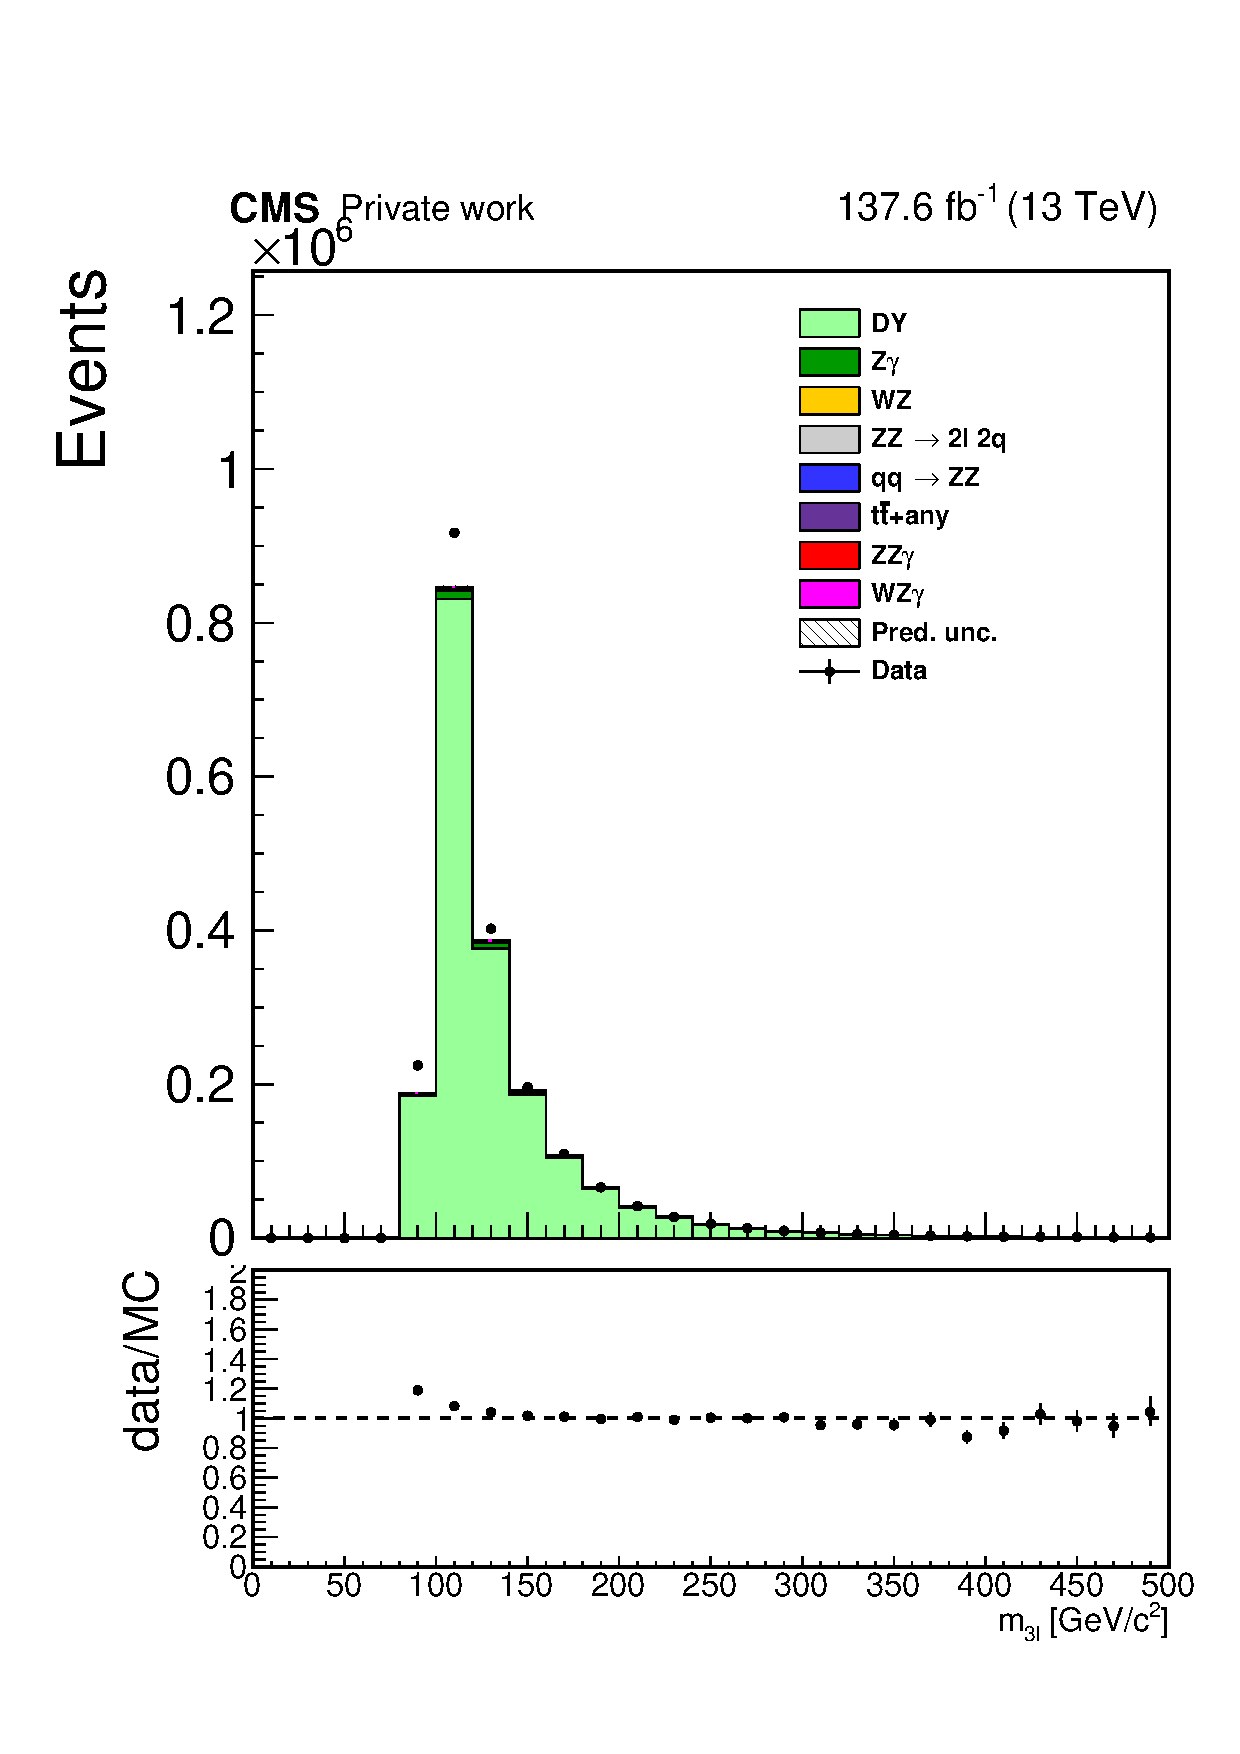
\includegraphics[width=.4\textwidth]{VVGammaAnalyzer/Run2/fullMC/CRLFR/ZL_mass_pow.pdf}}\quad
  \subfigure [] {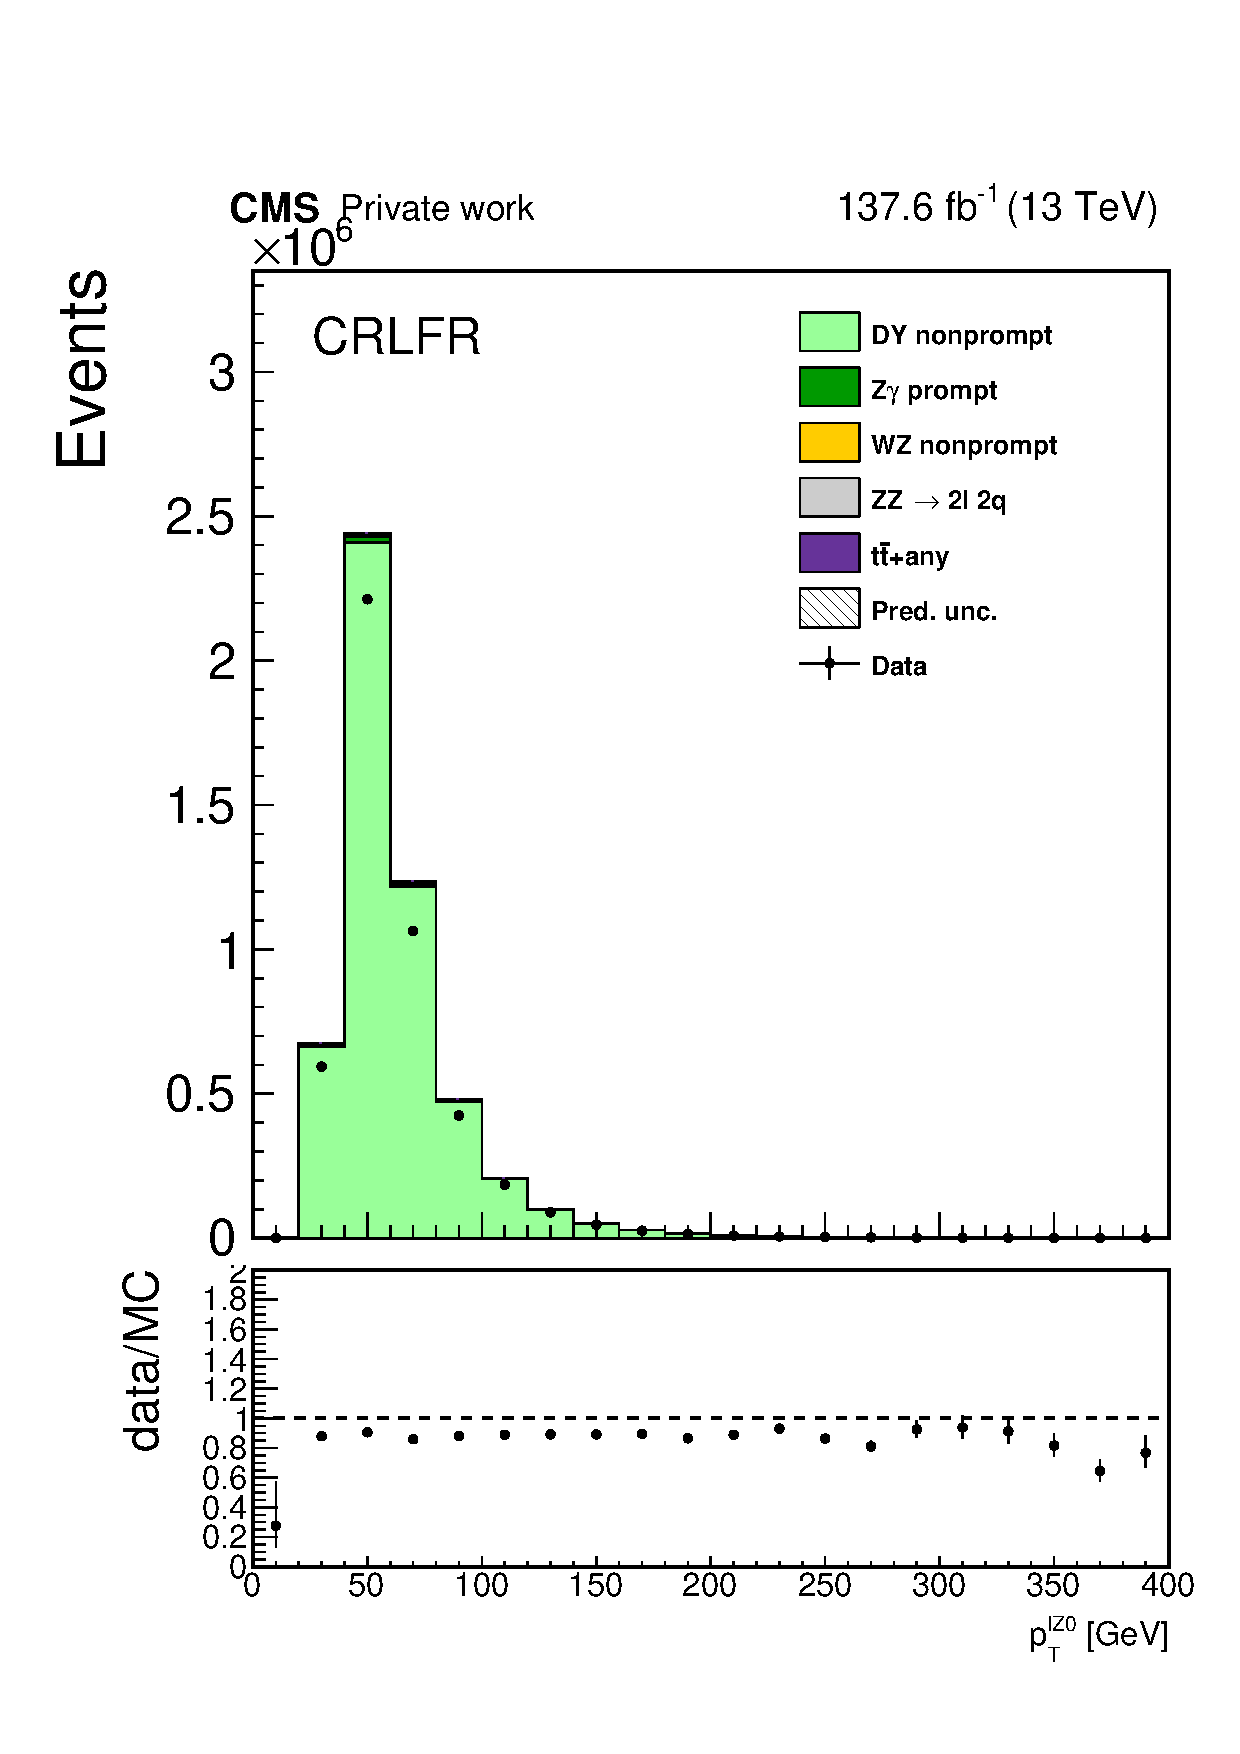
\includegraphics[width=.4\textwidth]{VVGammaAnalyzer/Run2/fullMC/CRLFR/Z_l0_pt_pow.pdf}}
  \caption{Invariant mass of the three lepton system and transverse momentum of the leading lepton from the Z candidate
  in the fake rate measurement region, integrated on the whole Run2 period.}
  \label{fig:CRLFR_inclusive}
\end{figure}

\begin{figure}
  \centering
  \subfigure [] {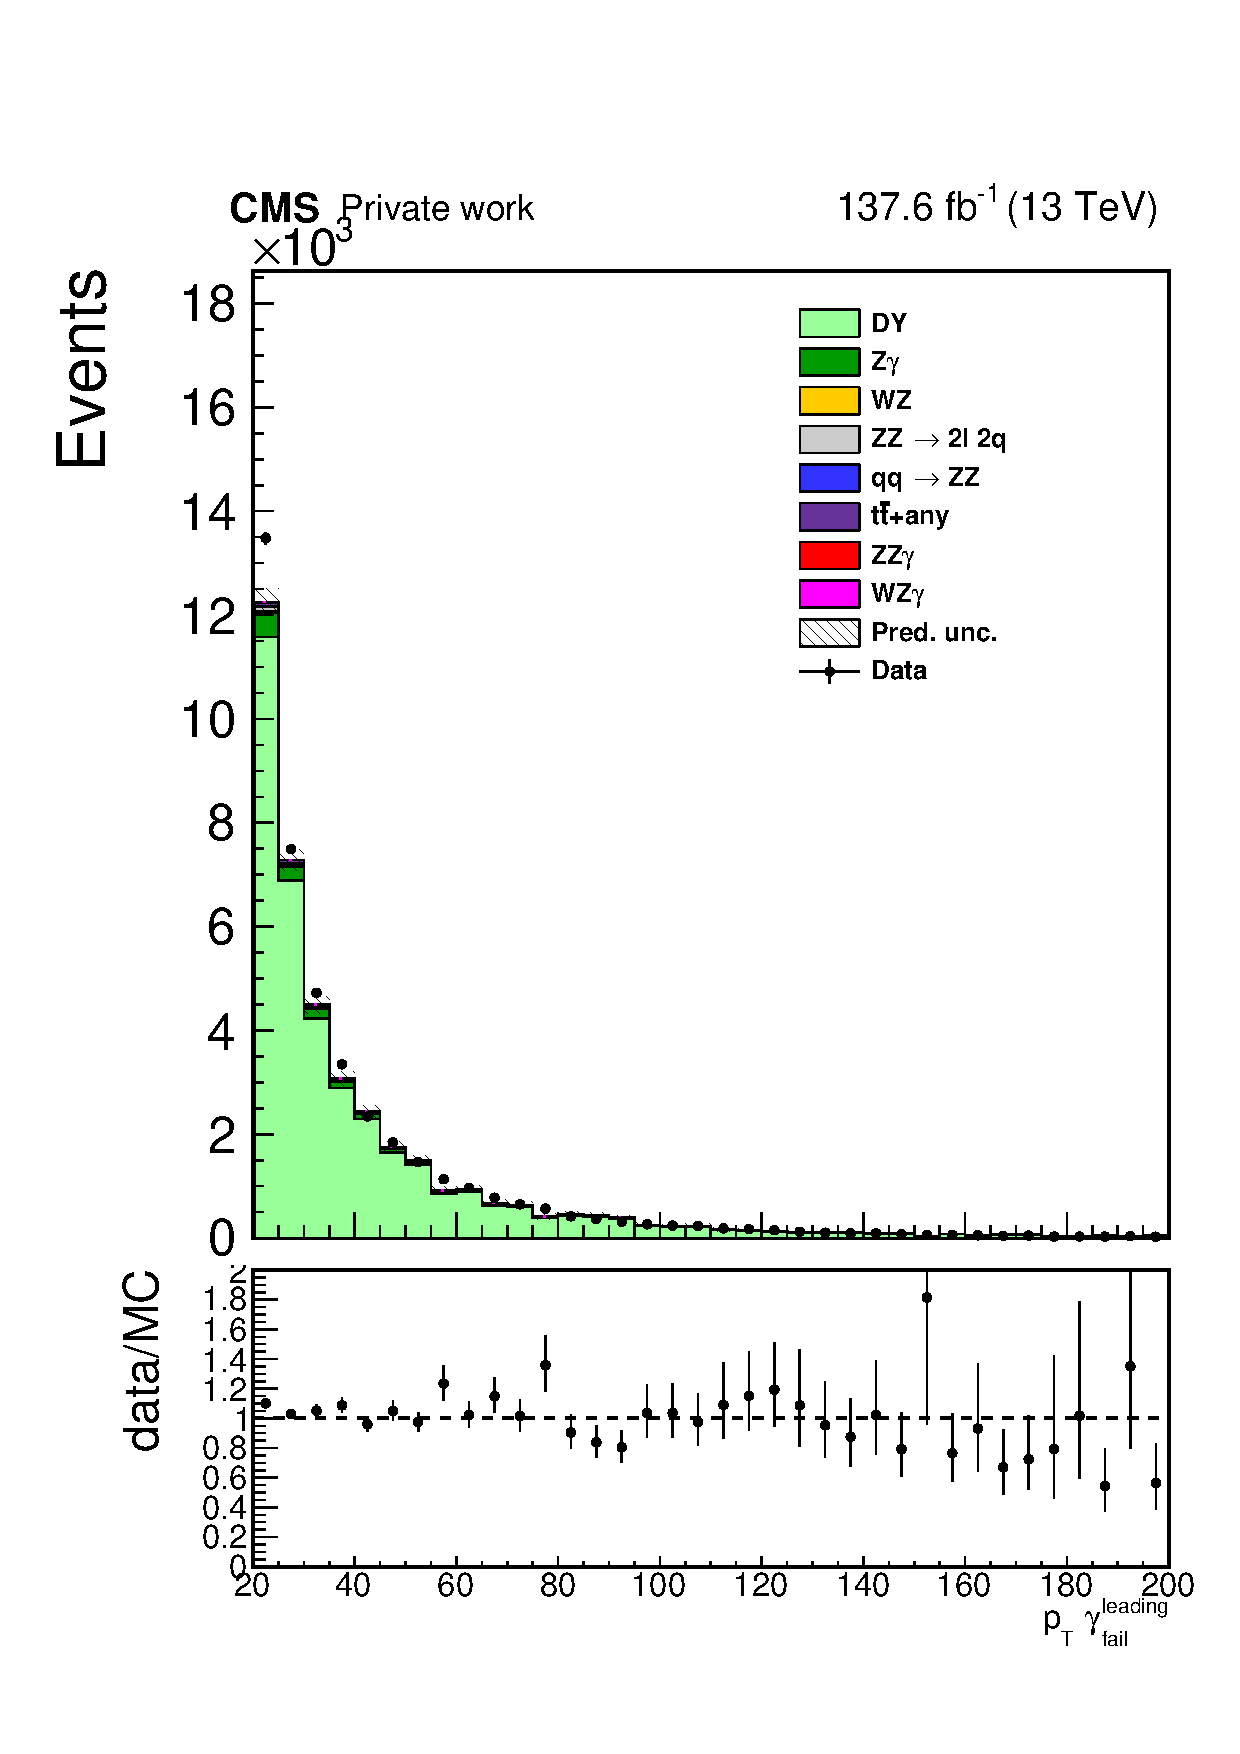
\includegraphics[width=.4\textwidth]{VVGammaAnalyzer/Run2/fullMC/CRLFR/lead_fail_pt_fine_pow.pdf}}\quad
  \subfigure [] {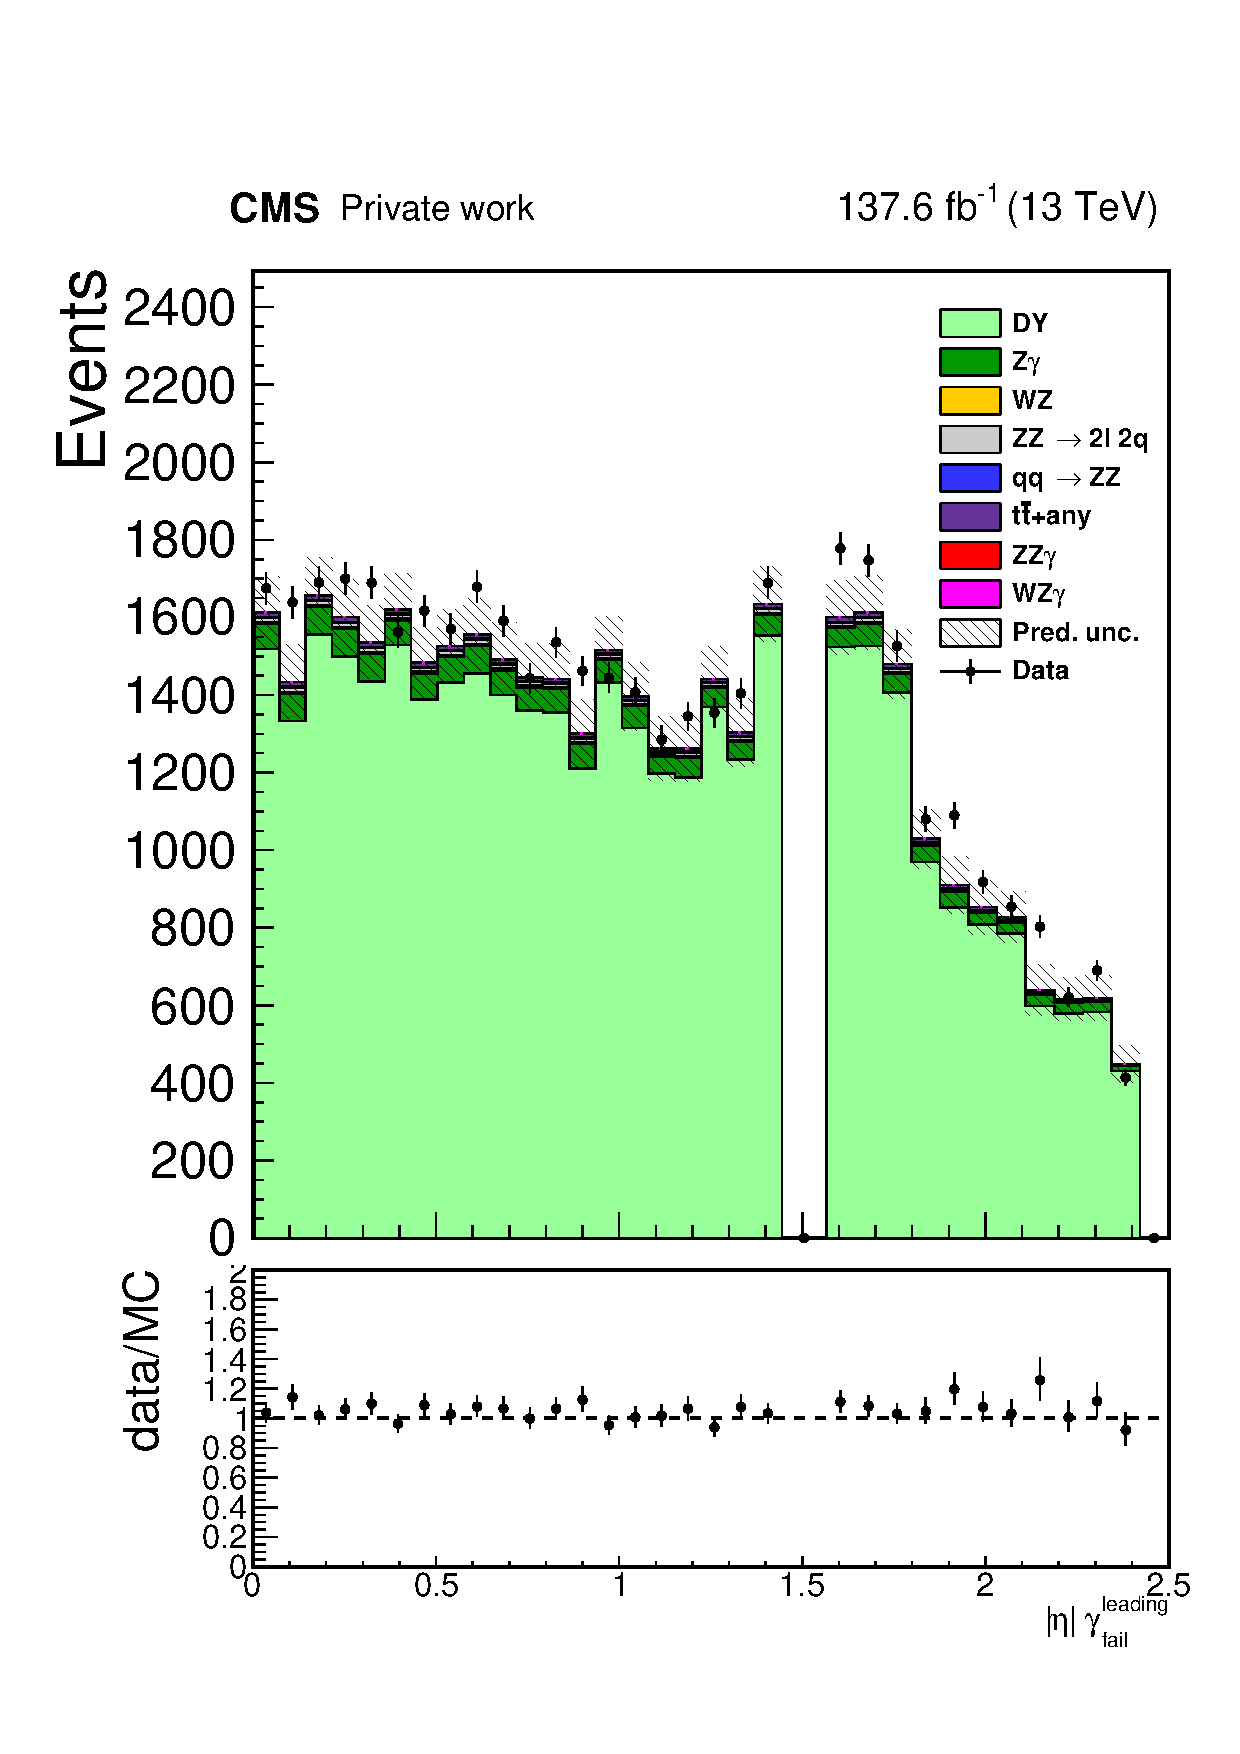
\includegraphics[width=.4\textwidth]{VVGammaAnalyzer/Run2/fullMC/CRLFR/lead_fail_aeta_fine_pow.pdf}}
  \caption{Transverse momentum and pseudorapidity of photons passing the loose criterion (VeryLoose ID) but failing the tight selection (Loose working point of the cut-based ID)
    in the fake rate measurement region, integrated on the whole Run2 period.}
  \label{fig:CRLFR_lead_fail}
\end{figure}

\begin{figure}
  \centering
  \subfigure [] {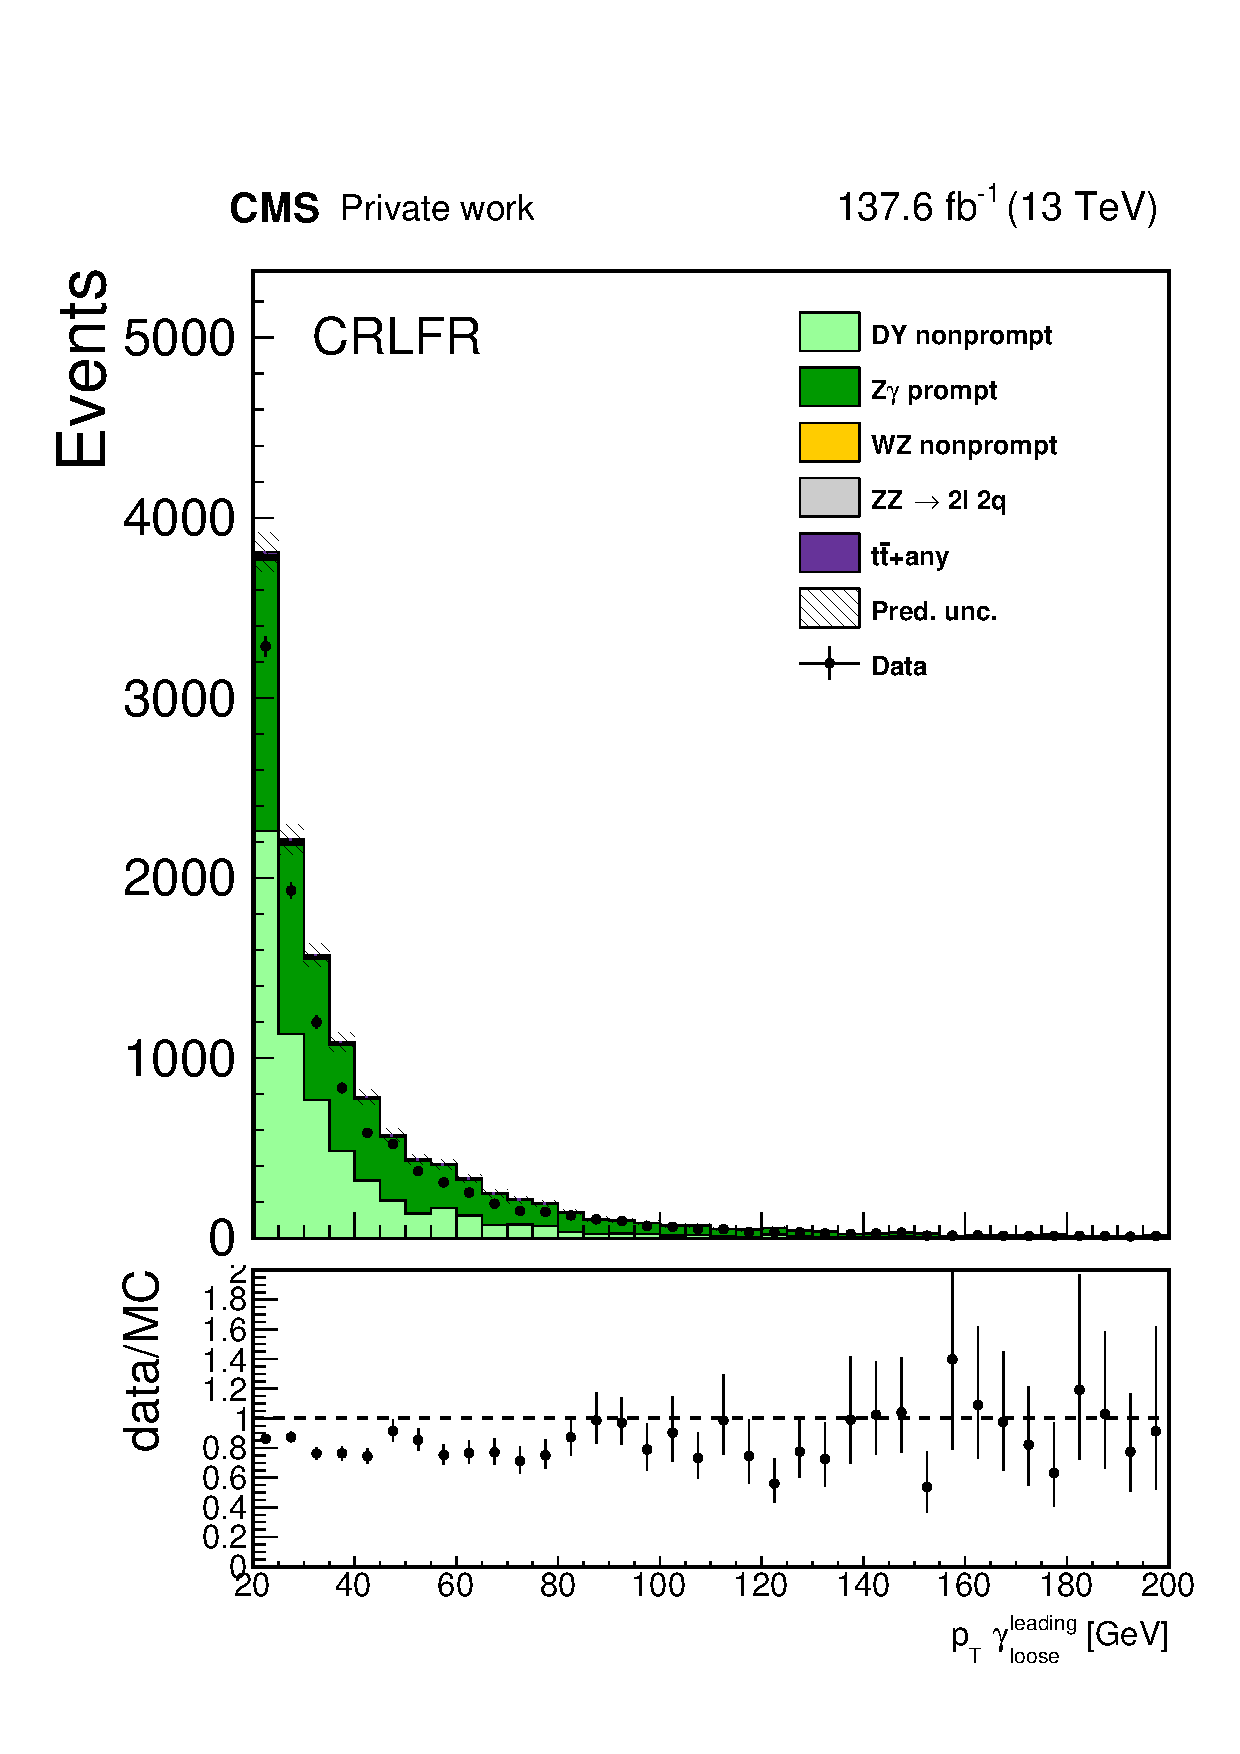
\includegraphics[width=.4\textwidth]{VVGammaAnalyzer/Run2/fullMC/CRLFR/lead_loose_pt_fine_pow.pdf}}\quad
  \subfigure [] {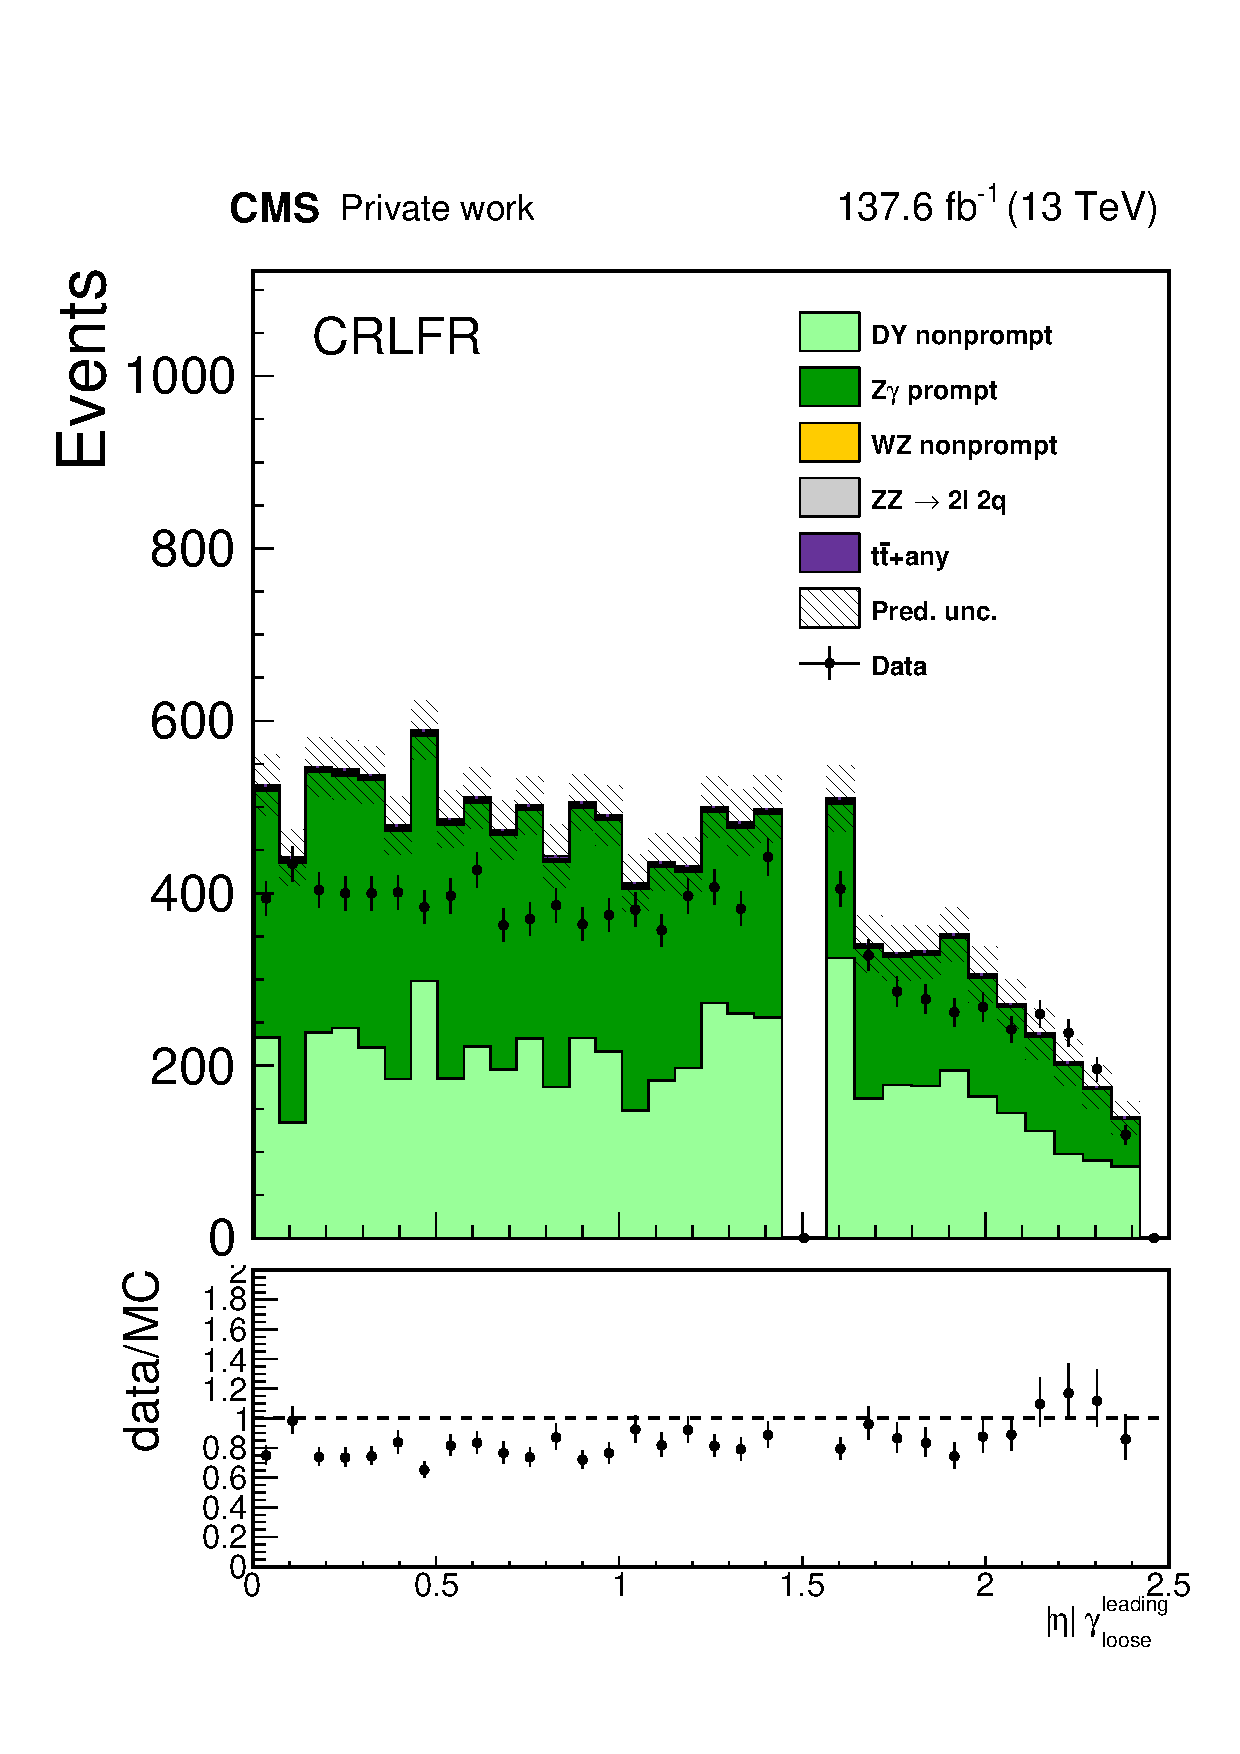
\includegraphics[width=.4\textwidth]{VVGammaAnalyzer/Run2/fullMC/CRLFR/lead_loose_aeta_fine_pow.pdf}}
  \caption{Transverse momentum and pseudorapidity of photons passing the tight selection (Loose working point of the cut-based ID)
    in the fake rate measurement region, integrated on the whole Run2 period.}
  \label{fig:CRLFR_lead_pass}
\end{figure}

The fake rate is then measured as the ratio of events in which the photon passes also the tight selection (the Loose working point of the cut-based ID)
to the total.
This measurement is done separately for endcap and barrel, for several bins of \pt (Figure \ref{fig:phFR_VLtoL}).

\begin{figure}
\subfigure [2016preVFP ] {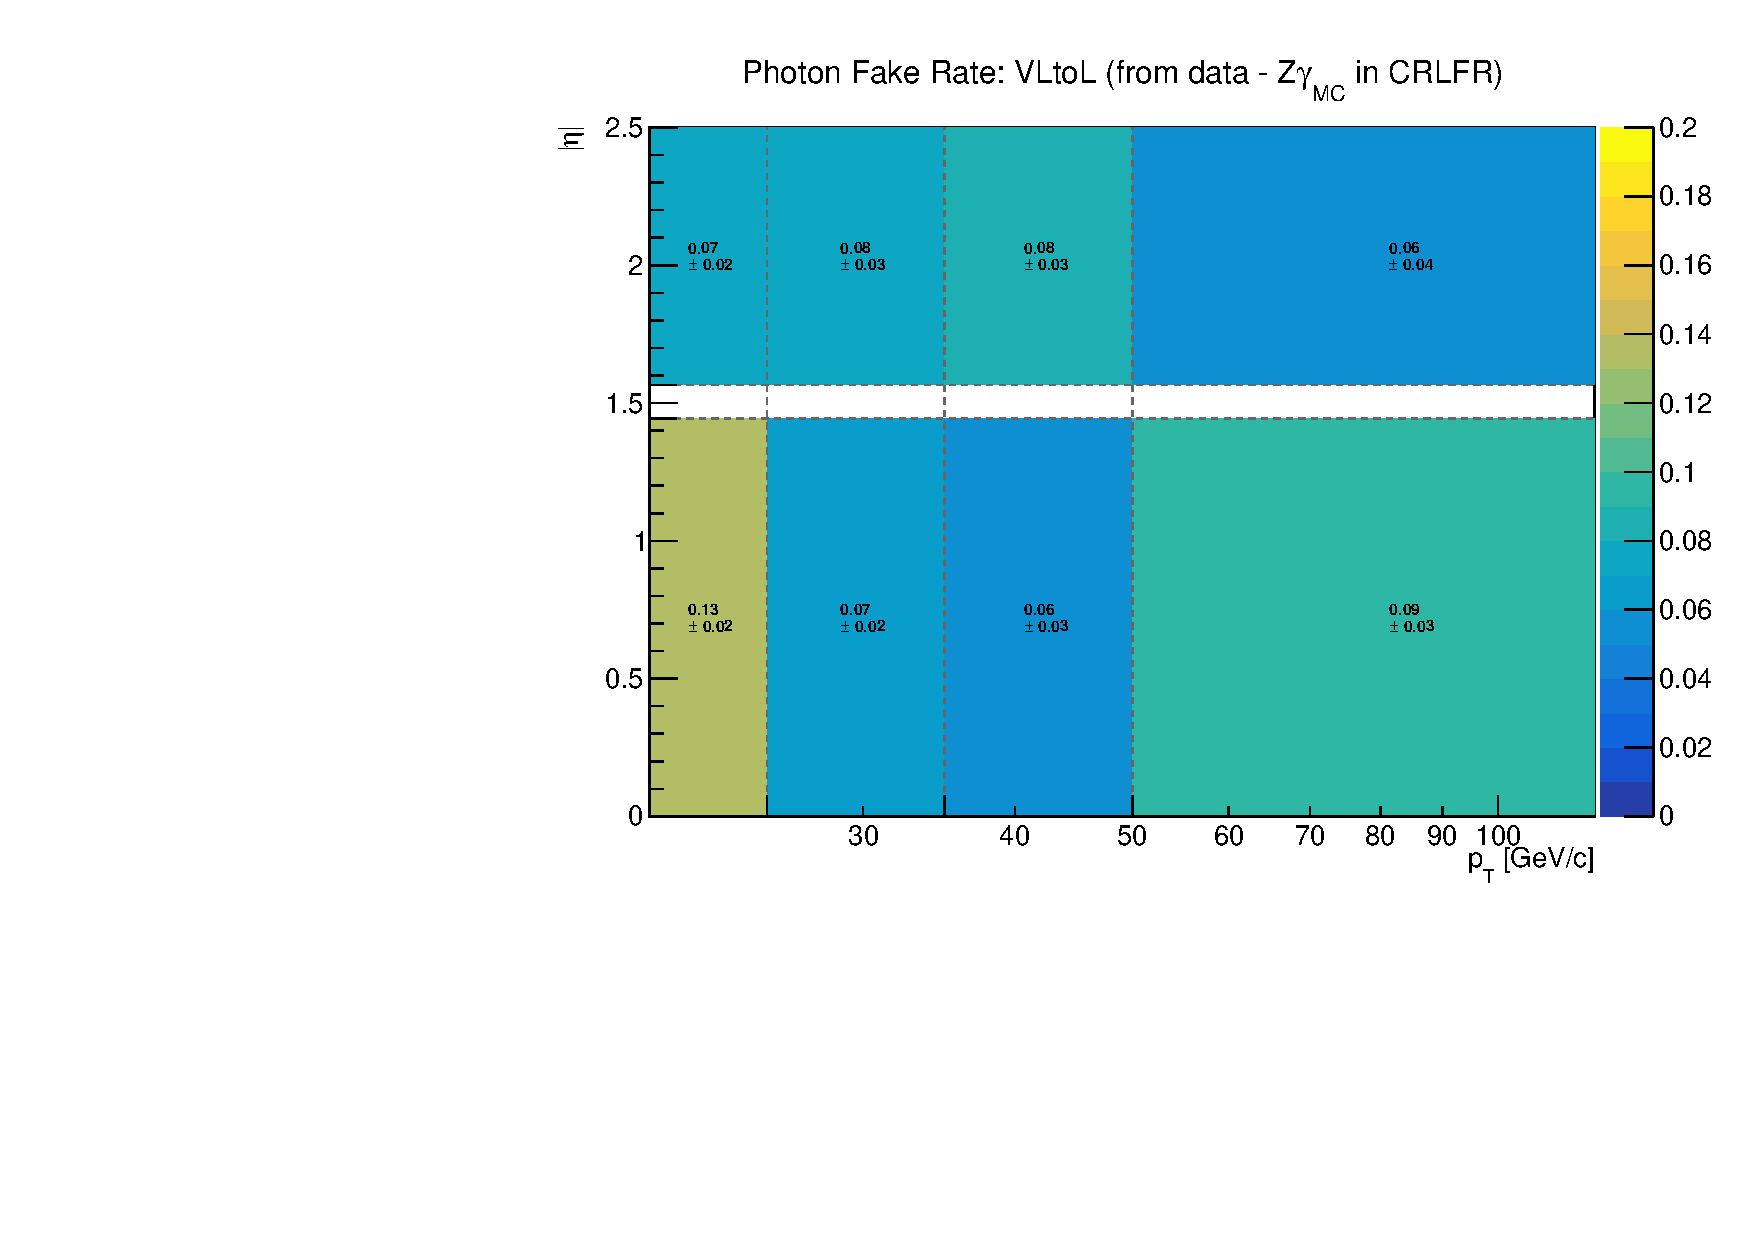
\includegraphics[width=.5\textwidth]{Figures/FR_VLtoL_pt-aeta_data-ZGToLLG_2016preVFP.pdf}}%
\subfigure [2016postVFP] {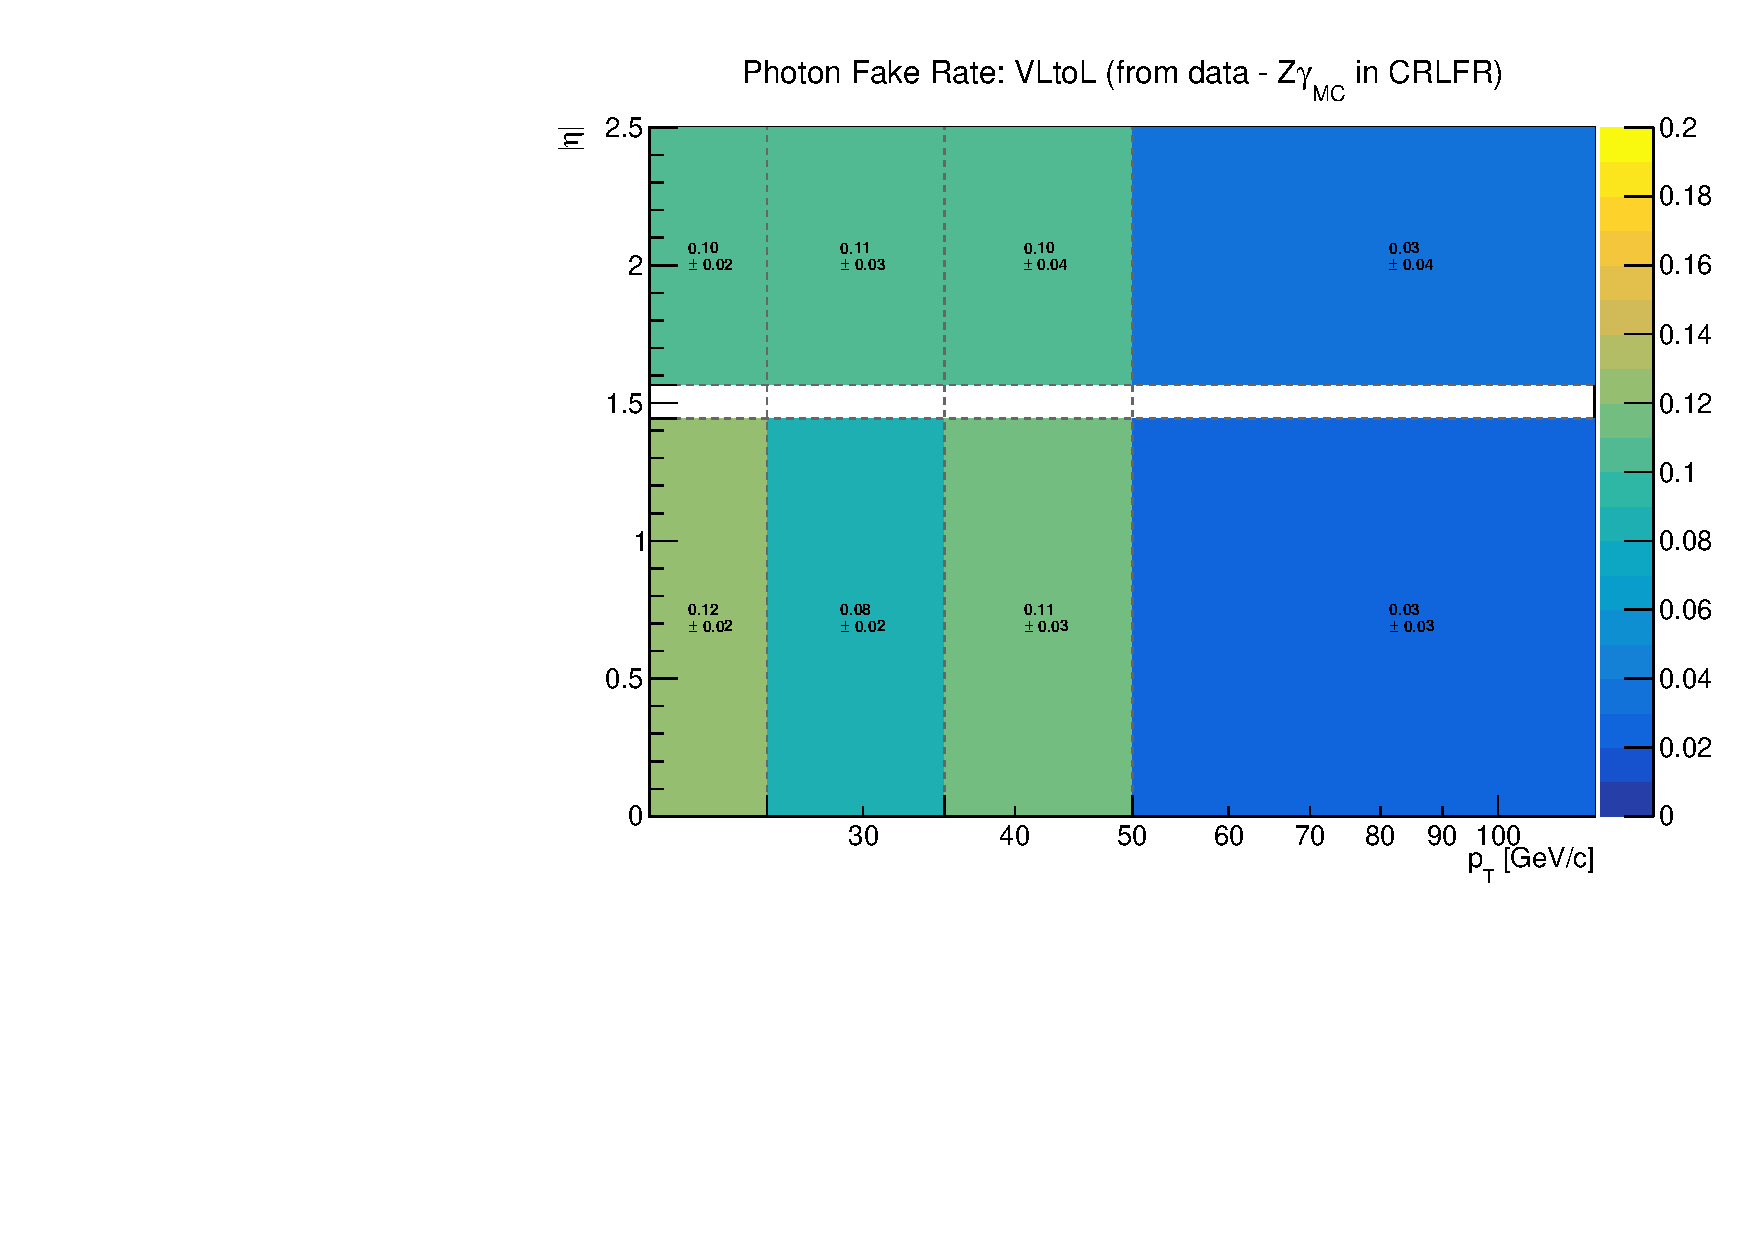
\includegraphics[width=.5\textwidth]{Figures/FR_VLtoL_pt-aeta_data-ZGToLLG_2016postVFP.pdf}}\\
\subfigure [2017]        {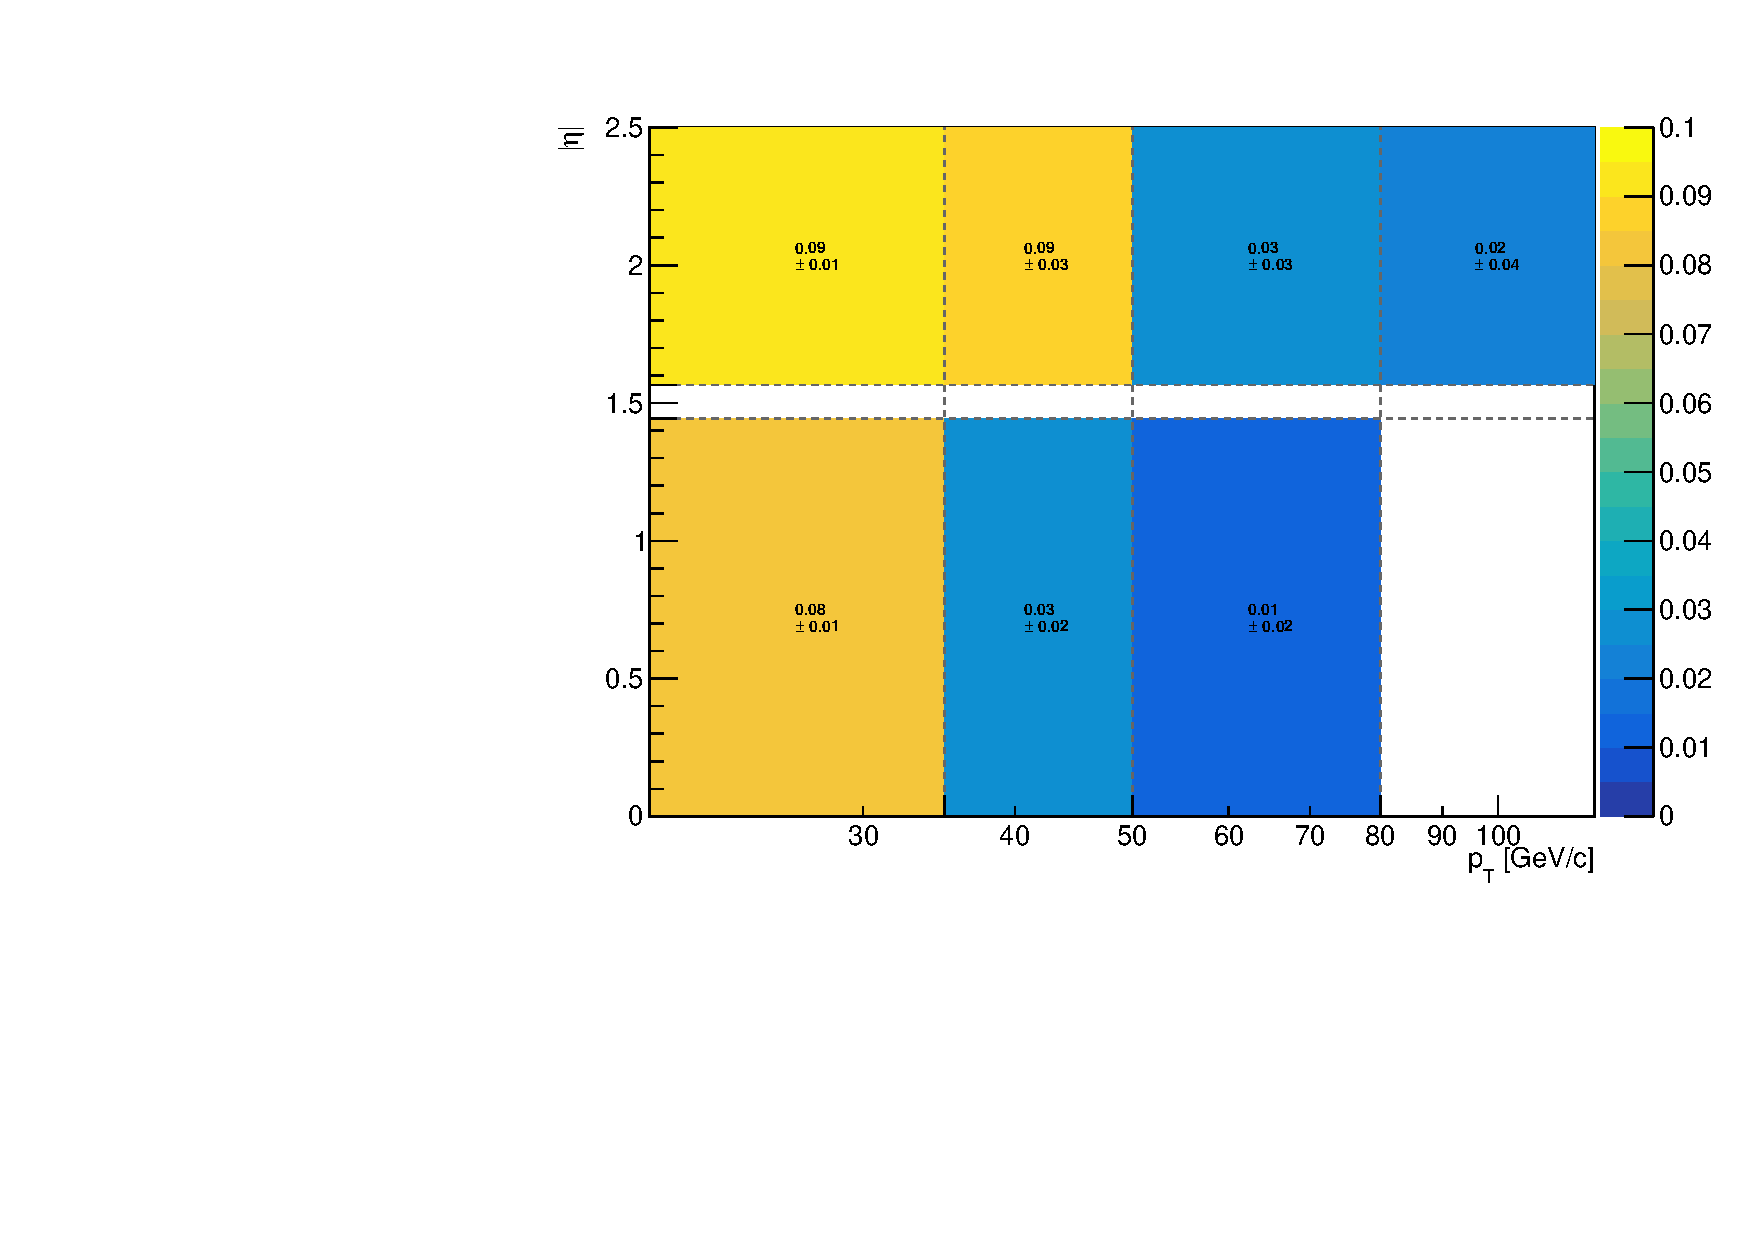
\includegraphics[width=.5\textwidth]{Figures/FR_VLtoL_pt-aeta_data-ZGToLLG_2017.pdf}}%
\subfigure [2018]        {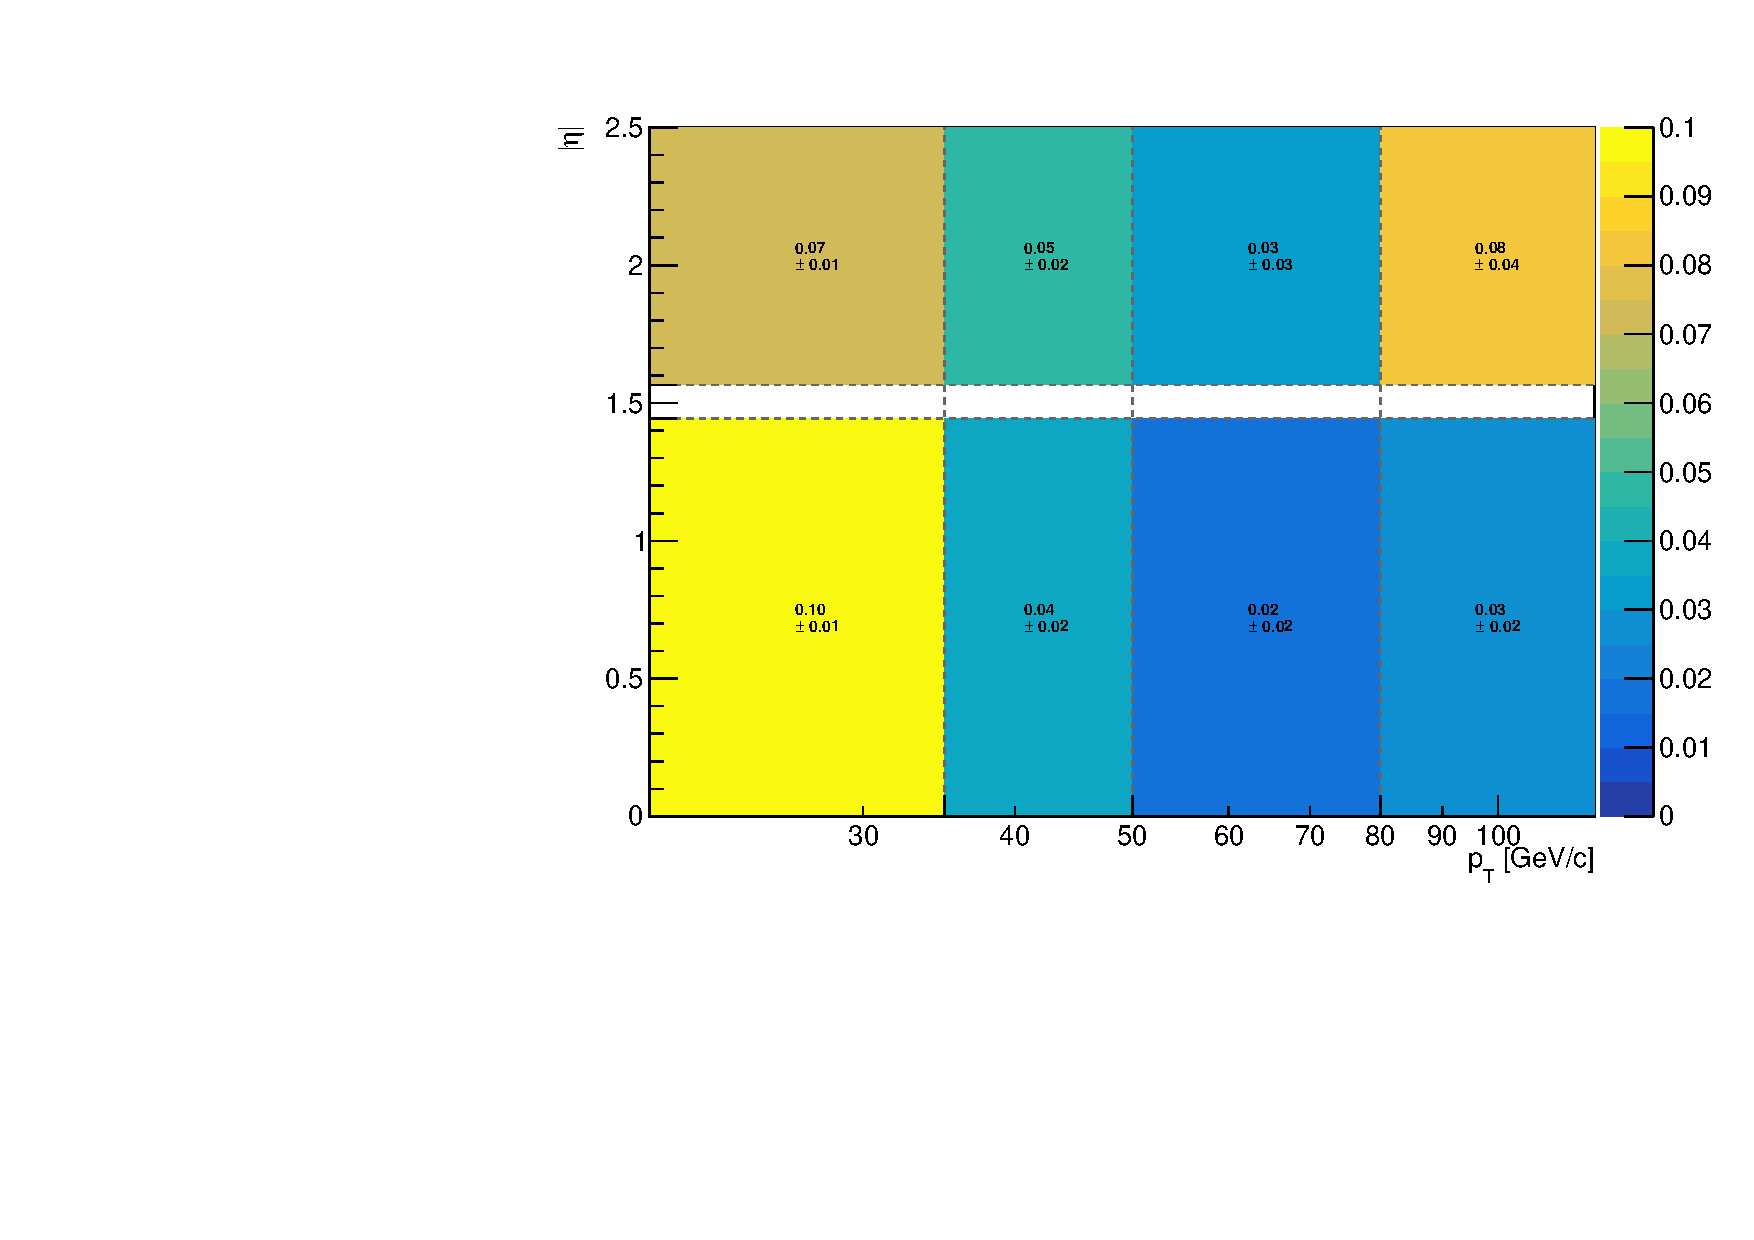
\includegraphics[width=.5\textwidth]{Figures/FR_VLtoL_pt-aeta_data-ZGToLLG_2018.pdf}}
\caption{Photon non-prompt rate as measured in data (with prompt $Z\gamma$ subtraction) using the cut-based ID for the photon.}
\label{fig:phFR_VLtoL}
\end{figure}

To ensure the stability of the measurement against other variables in the event,
additional measurements are carried out in specific sub-regions, and the results compared.
In particular, the effect of:
\begin{itemize}
\item The status of the third lepton: whether it passes or fails the tight selection.
  This could bias the measurement if the lepton were a misidentified jet and the additional hadronic activity produced an additional \nonprompt photon.
\item The flavour of the third lepton
\item The flavour of the SFOS pair that constitute the \PZ boson.
\item The number of additional jets in the event
\item The distance from the closest jet in the event
\end{itemize}

\note{Move to appendix? --> ``The results of these cross checks are in Appendix...''}

The photon non-prompt rate is assumed to be independent of the flavour of the leptons in the event.
This assumption is tested by deriving it separately for each flavour of the leptons of the Z boson $e^+ e^- \ell^\pm$ and $\mu^+ \mu^- \ell^\pm$, as shown in Figure \ref{fig:phFR_2e2m}.

\begin{figure}
\subfigure [$e^+ e^- \ell^\pm$]     {\resizebox{.5\textwidth}{!}{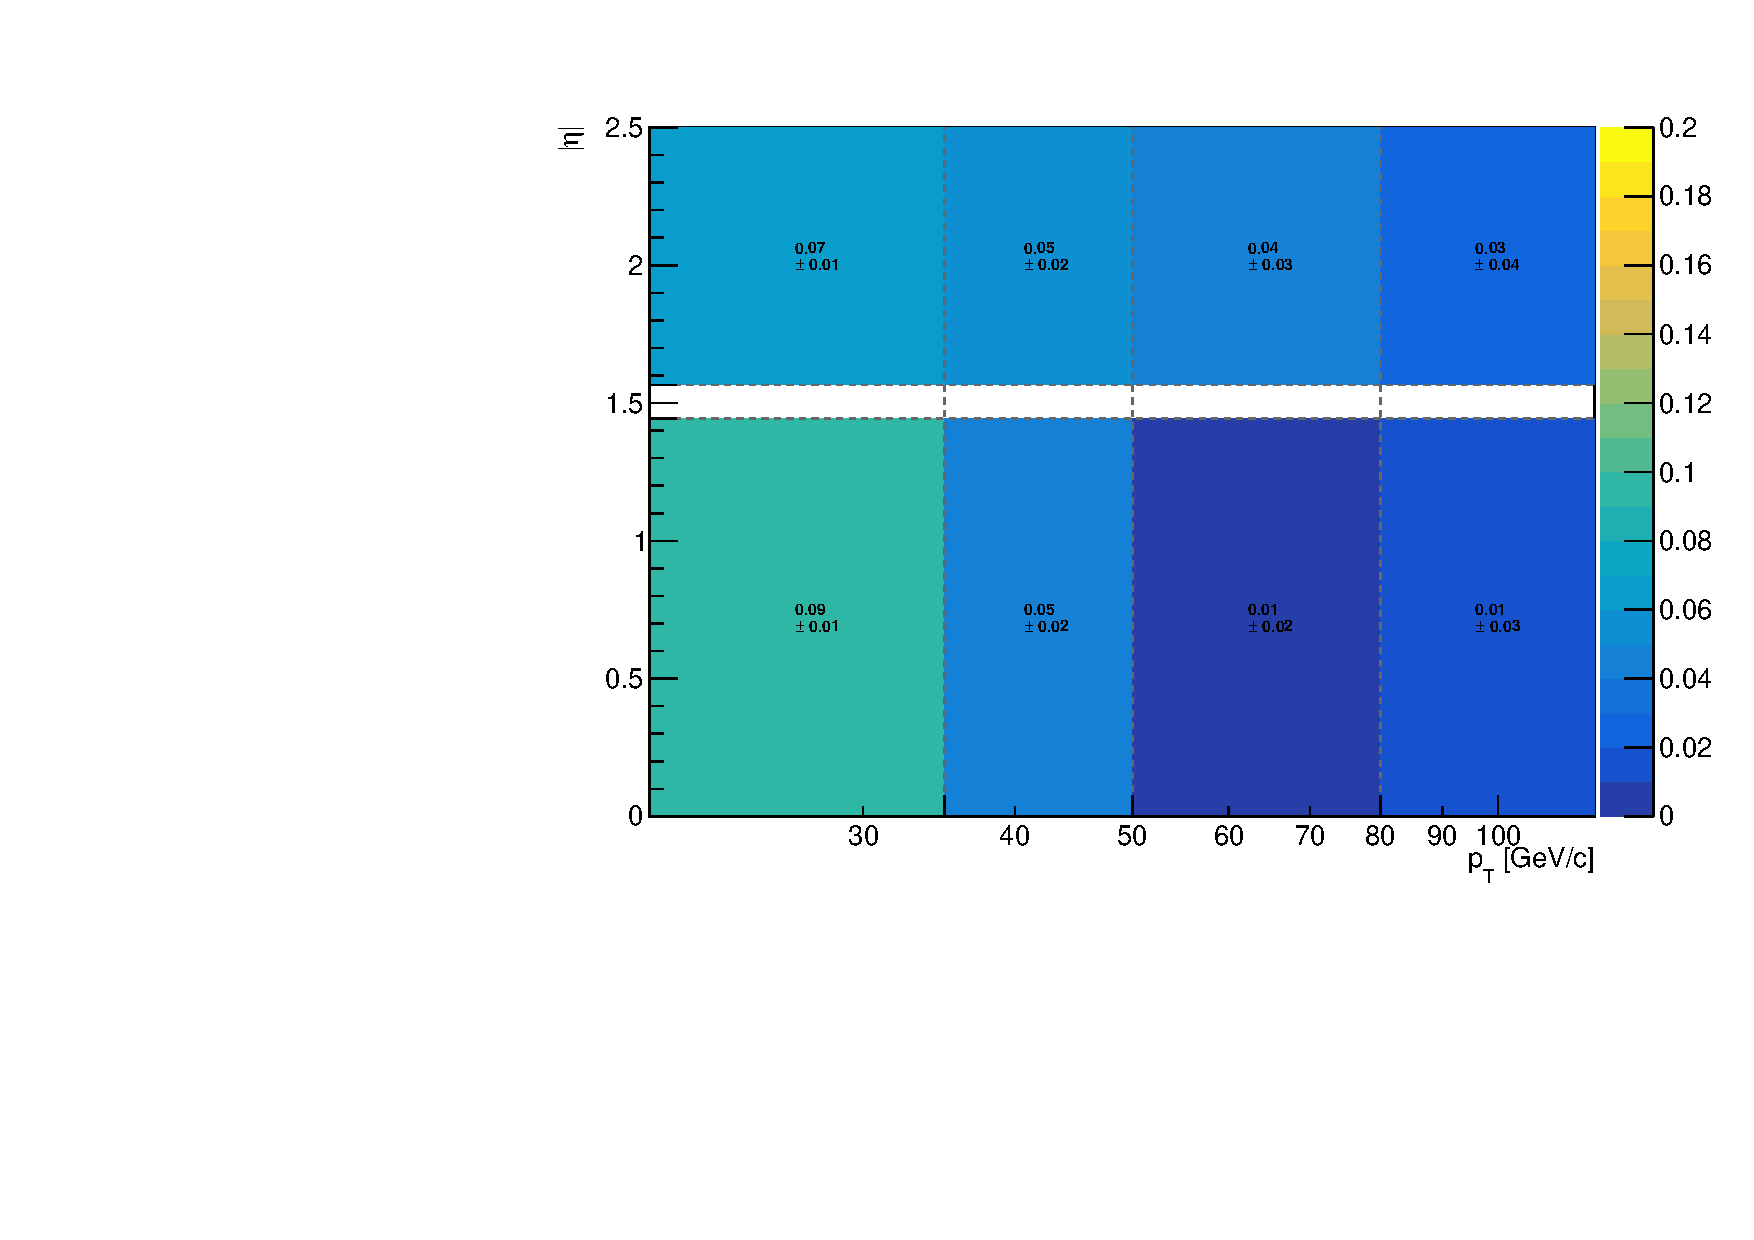
\includegraphics[width=.5\textwidth]{Figures/FR_VLtoL_pt-aeta_2e+x_data-ZGToLLG_2018.pdf}}}
\subfigure [$\mu^+ \mu^- \ell^\pm$] {\resizebox{.5\textwidth}{!}{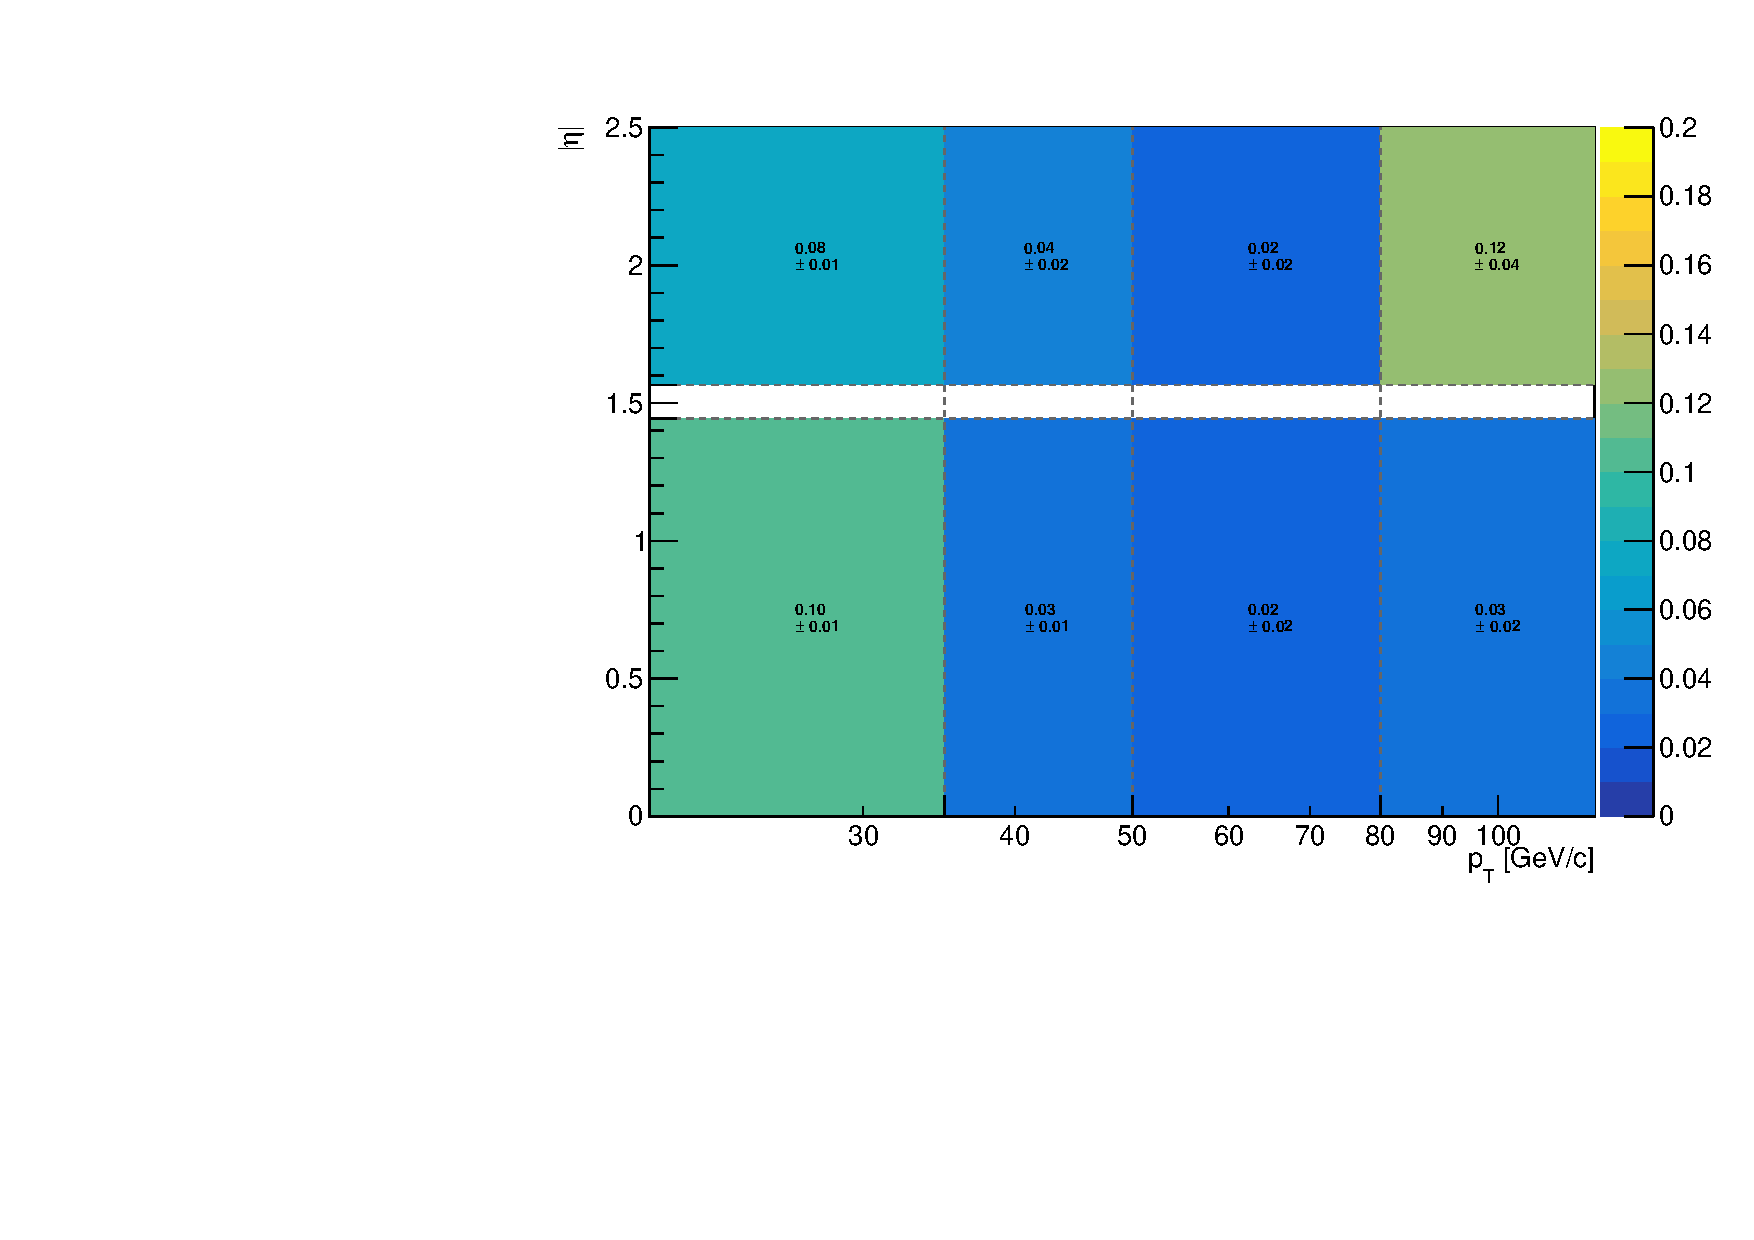
\includegraphics[width=.5\textwidth]{Figures/FR_VLtoL_pt-aeta_2m+x_data-ZGToLLG_2018.pdf}}}
\caption{Photon non-prompt rate as measured in 2018 data (with prompt $Z\gamma$ subtraction) in events with different lepton flavours for the Z boson.}
\label{fig:phFR_2e2m}
\end{figure}

The test is repeated for different flavours of the third lepton $\ell^+ \ell^- e^\pm$ and $\ell^+ \ell^- \mu^\pm$, and is shown in Figure \ref{fig:phFR_em}.

\begin{figure}
\subfigure [$\ell^+ \ell^- e^\pm$]   {\resizebox{.5\textwidth}{!}{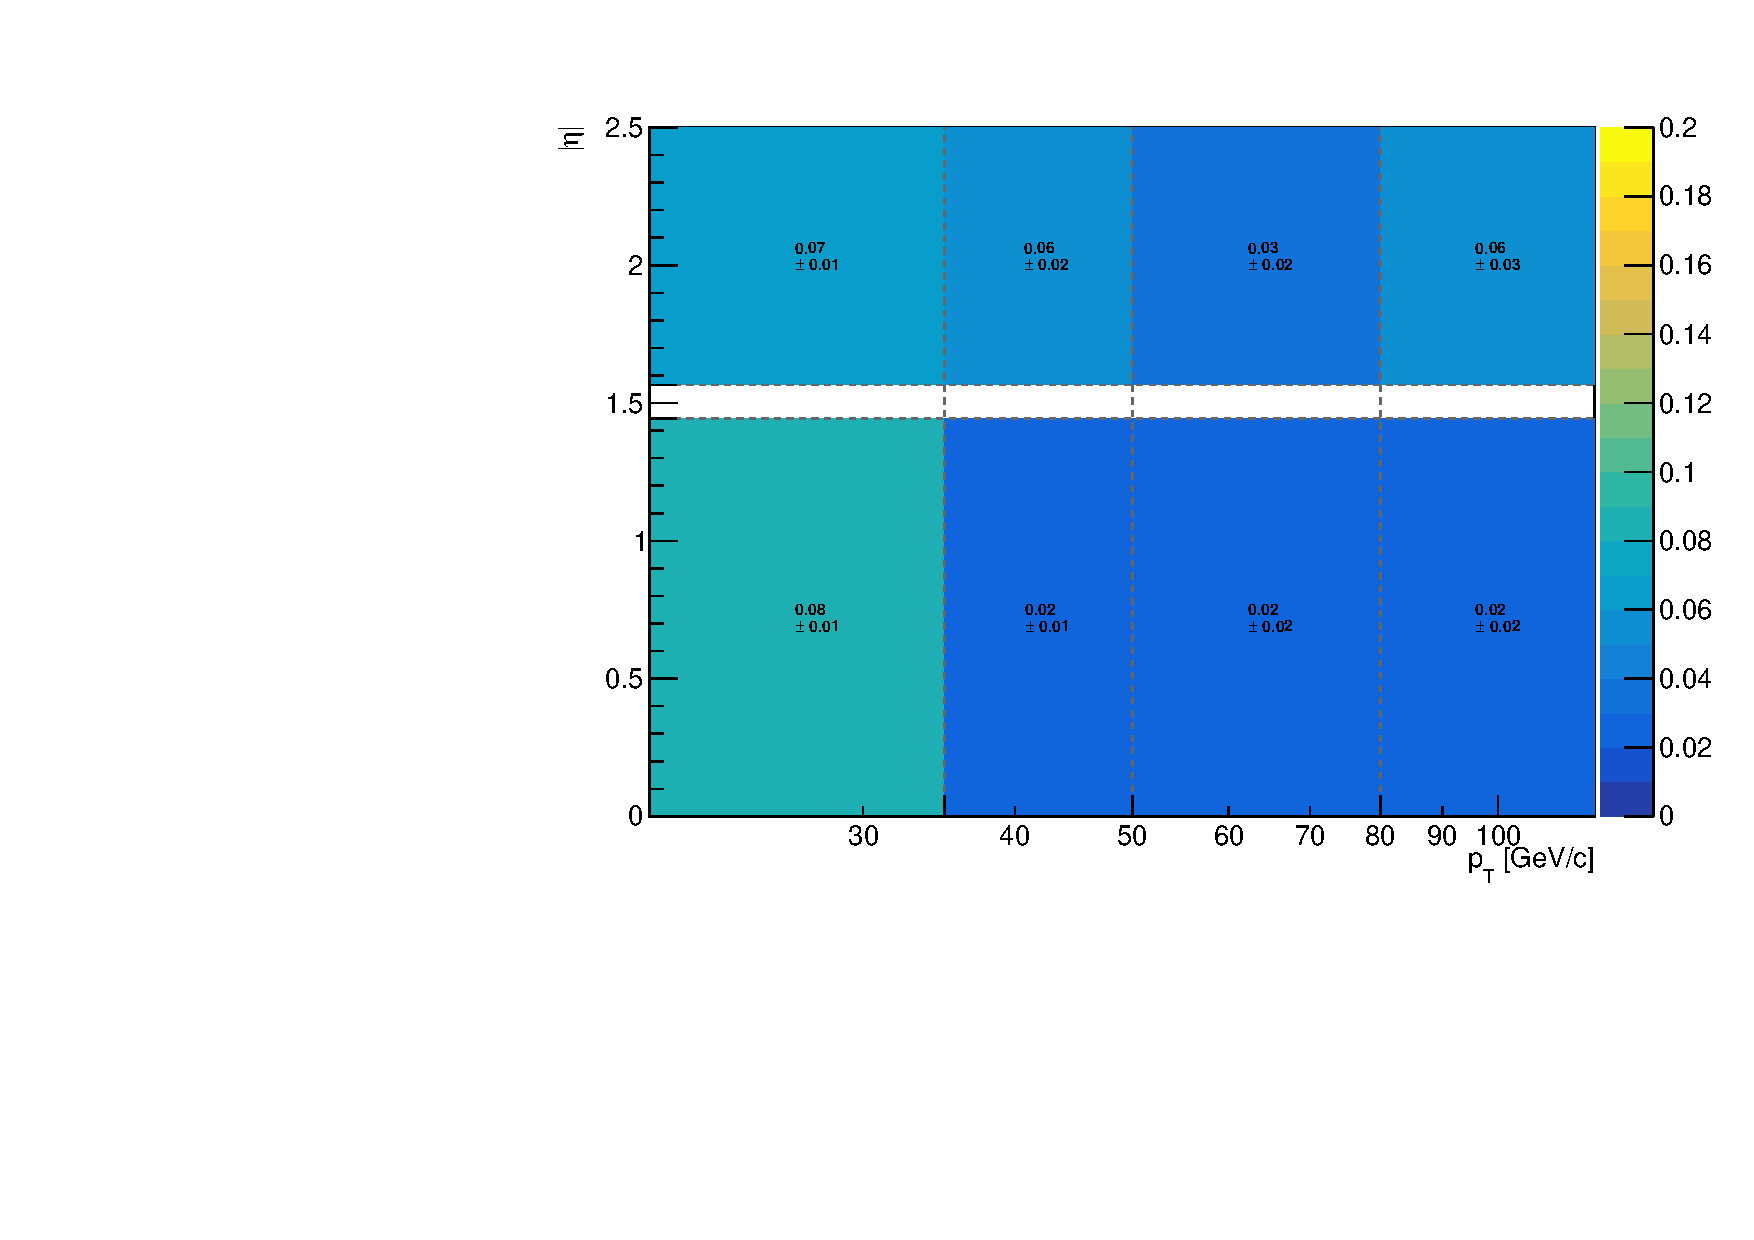
\includegraphics[width=.5\textwidth]{Figures/FR_VLtoL_pt-aeta_2x+e_data-ZGToLLG_2018.pdf}}}
\subfigure [$\ell^+ \ell^- \mu^\pm$] {\resizebox{.5\textwidth}{!}{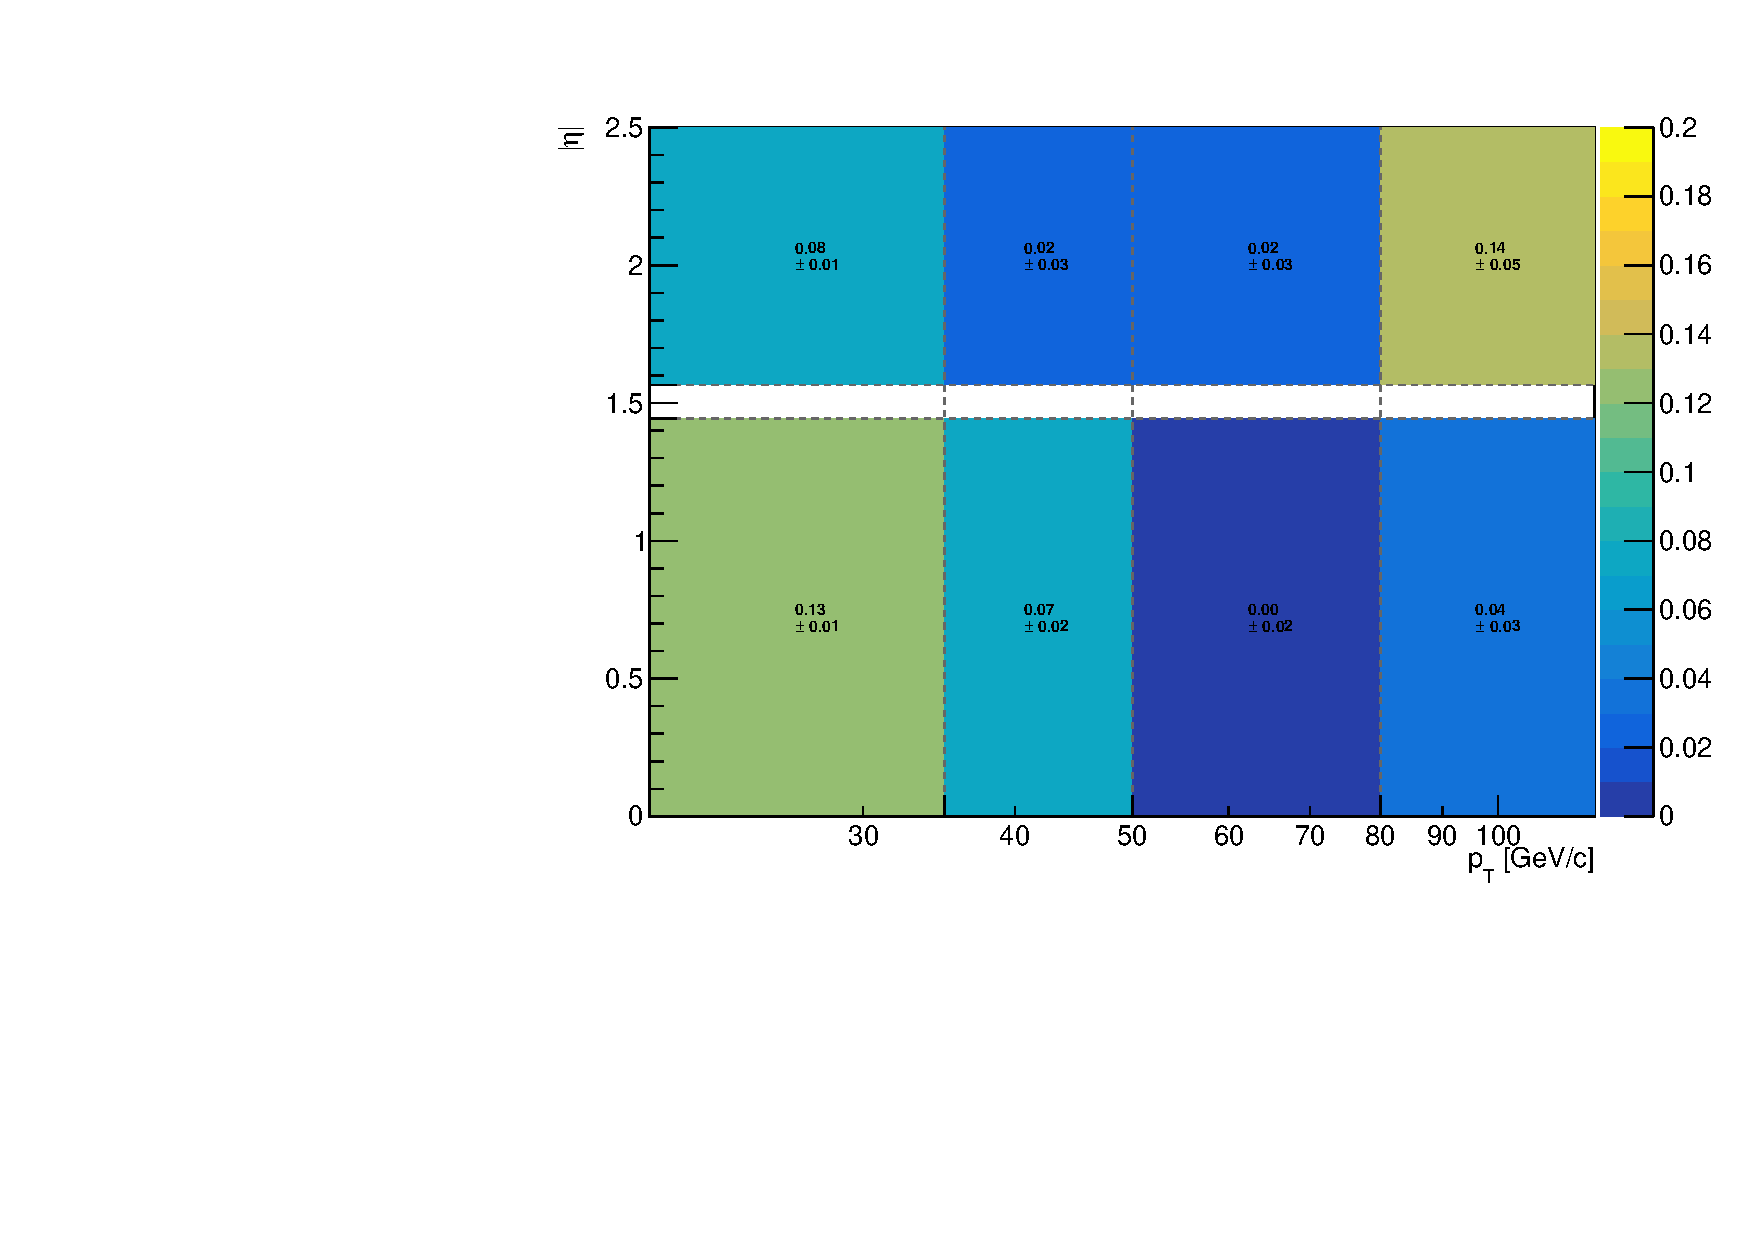
\includegraphics[width=.5\textwidth]{Figures/FR_VLtoL_pt-aeta_2x+m_data-ZGToLLG_2018.pdf}}}
\caption{Photon non-prompt rate as measured in 2018 data (with prompt $Z\gamma$ subtraction) in events with different flavours for the third lepton.}
\label{fig:phFR_em}
\end{figure}

Another test is performed by separating event where the third lepton passes/fails the tight analysis selection, shown in Figure \ref{fig:phFR_PF}.

\begin{figure}
\subfigure [$\ell^+ \ell^- \ell^\pm_{PASS}$] {\resizebox{.5\textwidth}{!}{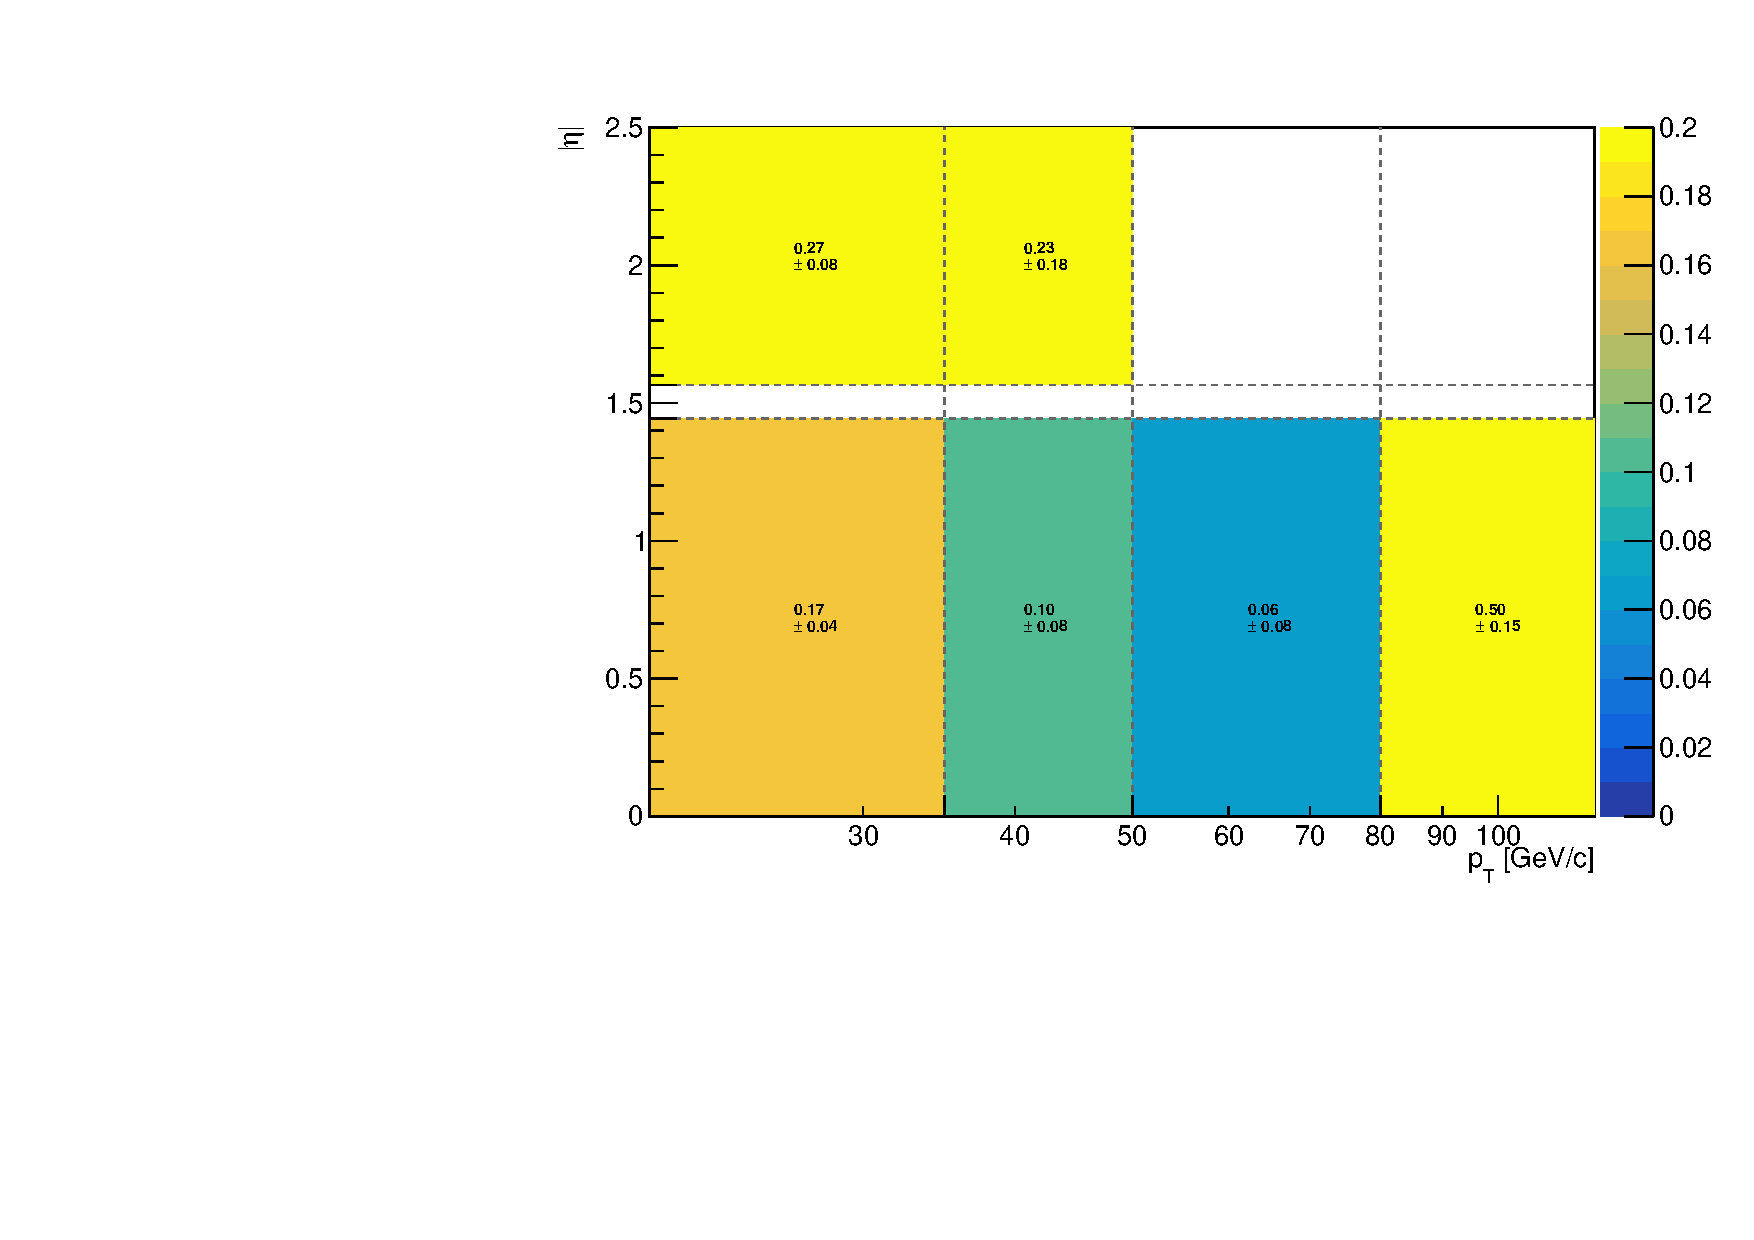
\includegraphics[width=.5\textwidth]{Figures/FR_VLtoL_pt-aeta_2x+P_data-ZGToLLG_2018.pdf}}}
\subfigure [$\ell^+ \ell^- \ell^\pm_{FAIL}$] {\resizebox{.5\textwidth}{!}{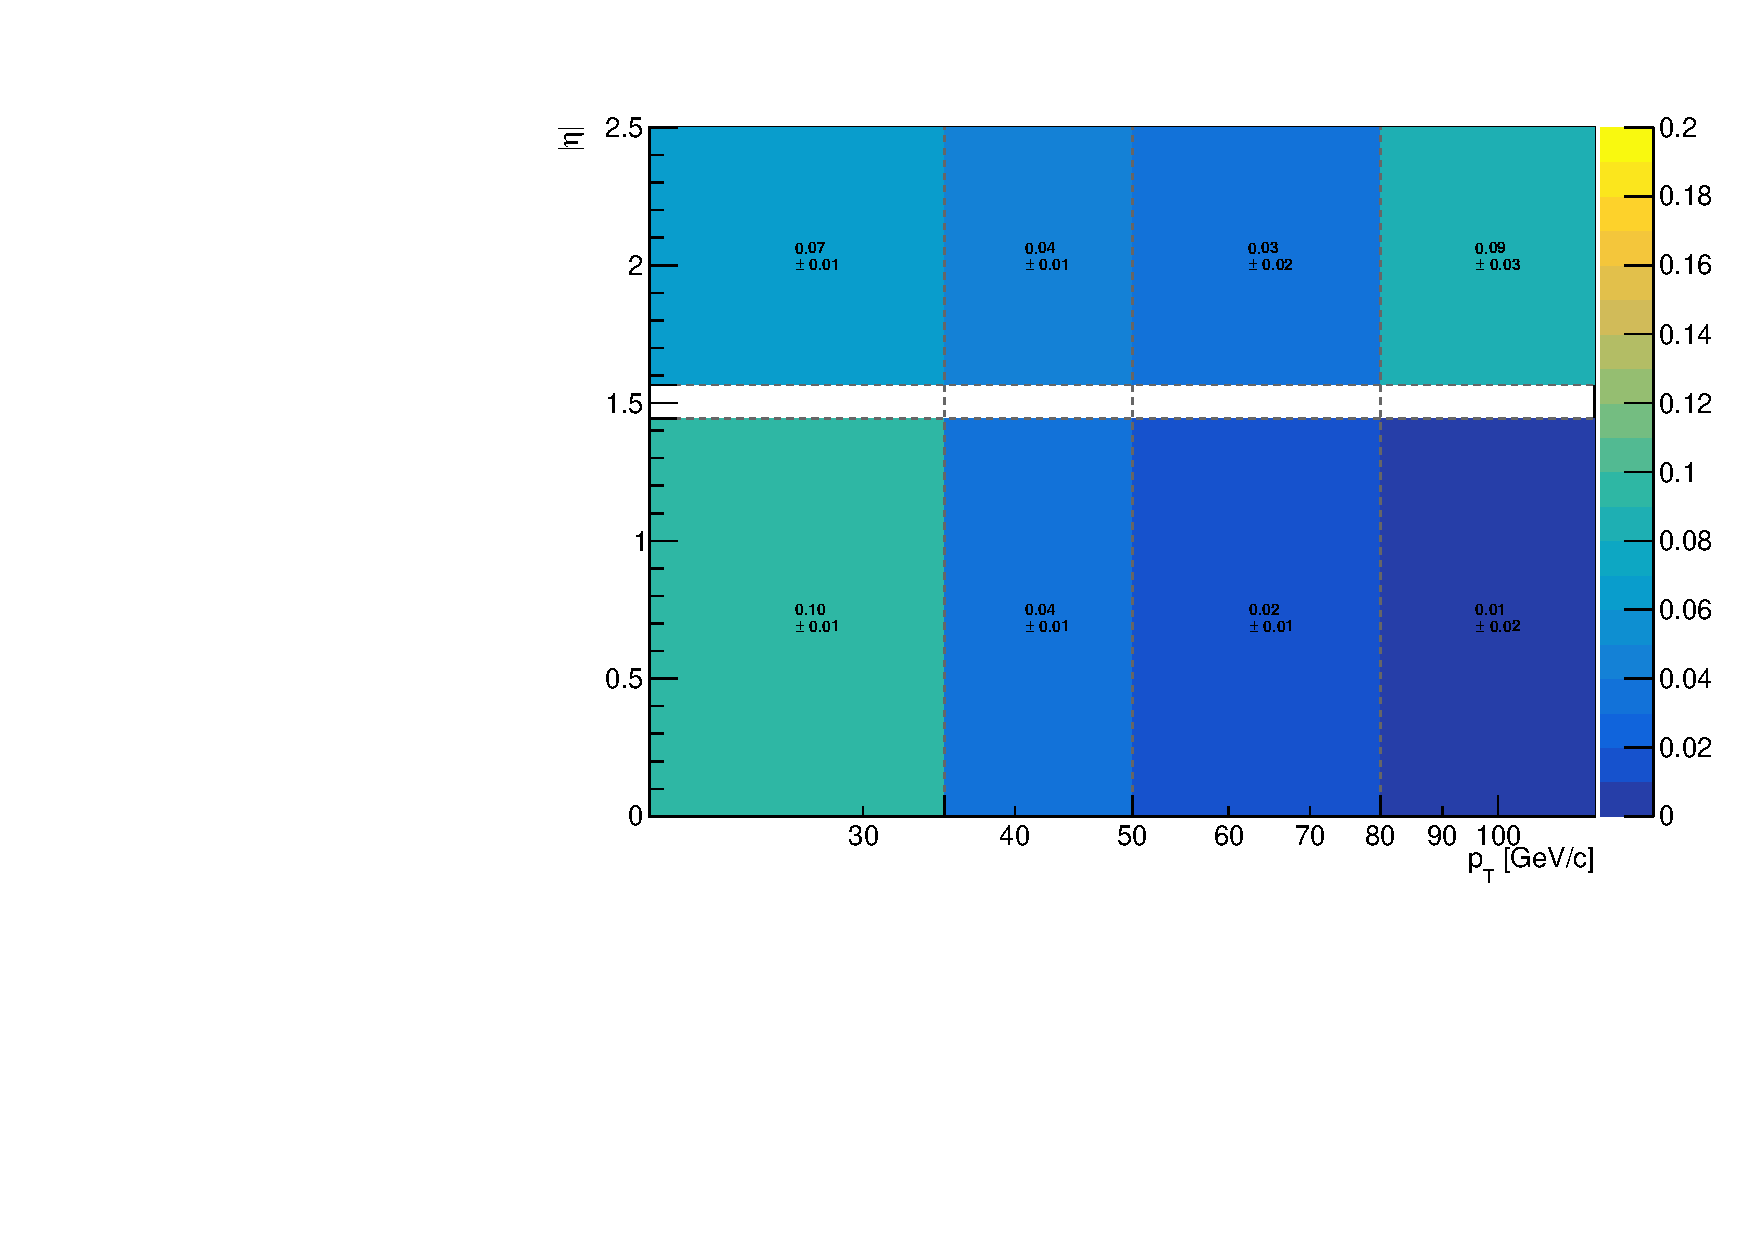
\includegraphics[width=.5\textwidth]{Figures/FR_VLtoL_pt-aeta_2x+F_data-ZGToLLG_2018.pdf}}}
\caption{Photon non-prompt rate as measured in 2018 data (with prompt $Z\gamma$ subtraction) in events where the third lepton passes/fails the tight selection, regardless of its flavour.}
\label{fig:phFR_PF}
\end{figure}

The trend for each $(p_{T}, |\eta|)$ bin for the different data-taking periods can be seen in Figure \ref{fig:phFR_time}.
It appears that, within the uncertainties, the measurements for each bin are compatible across the years and thus a single rate for the whole Run2 could be derived.

\begin{figure}
\centering
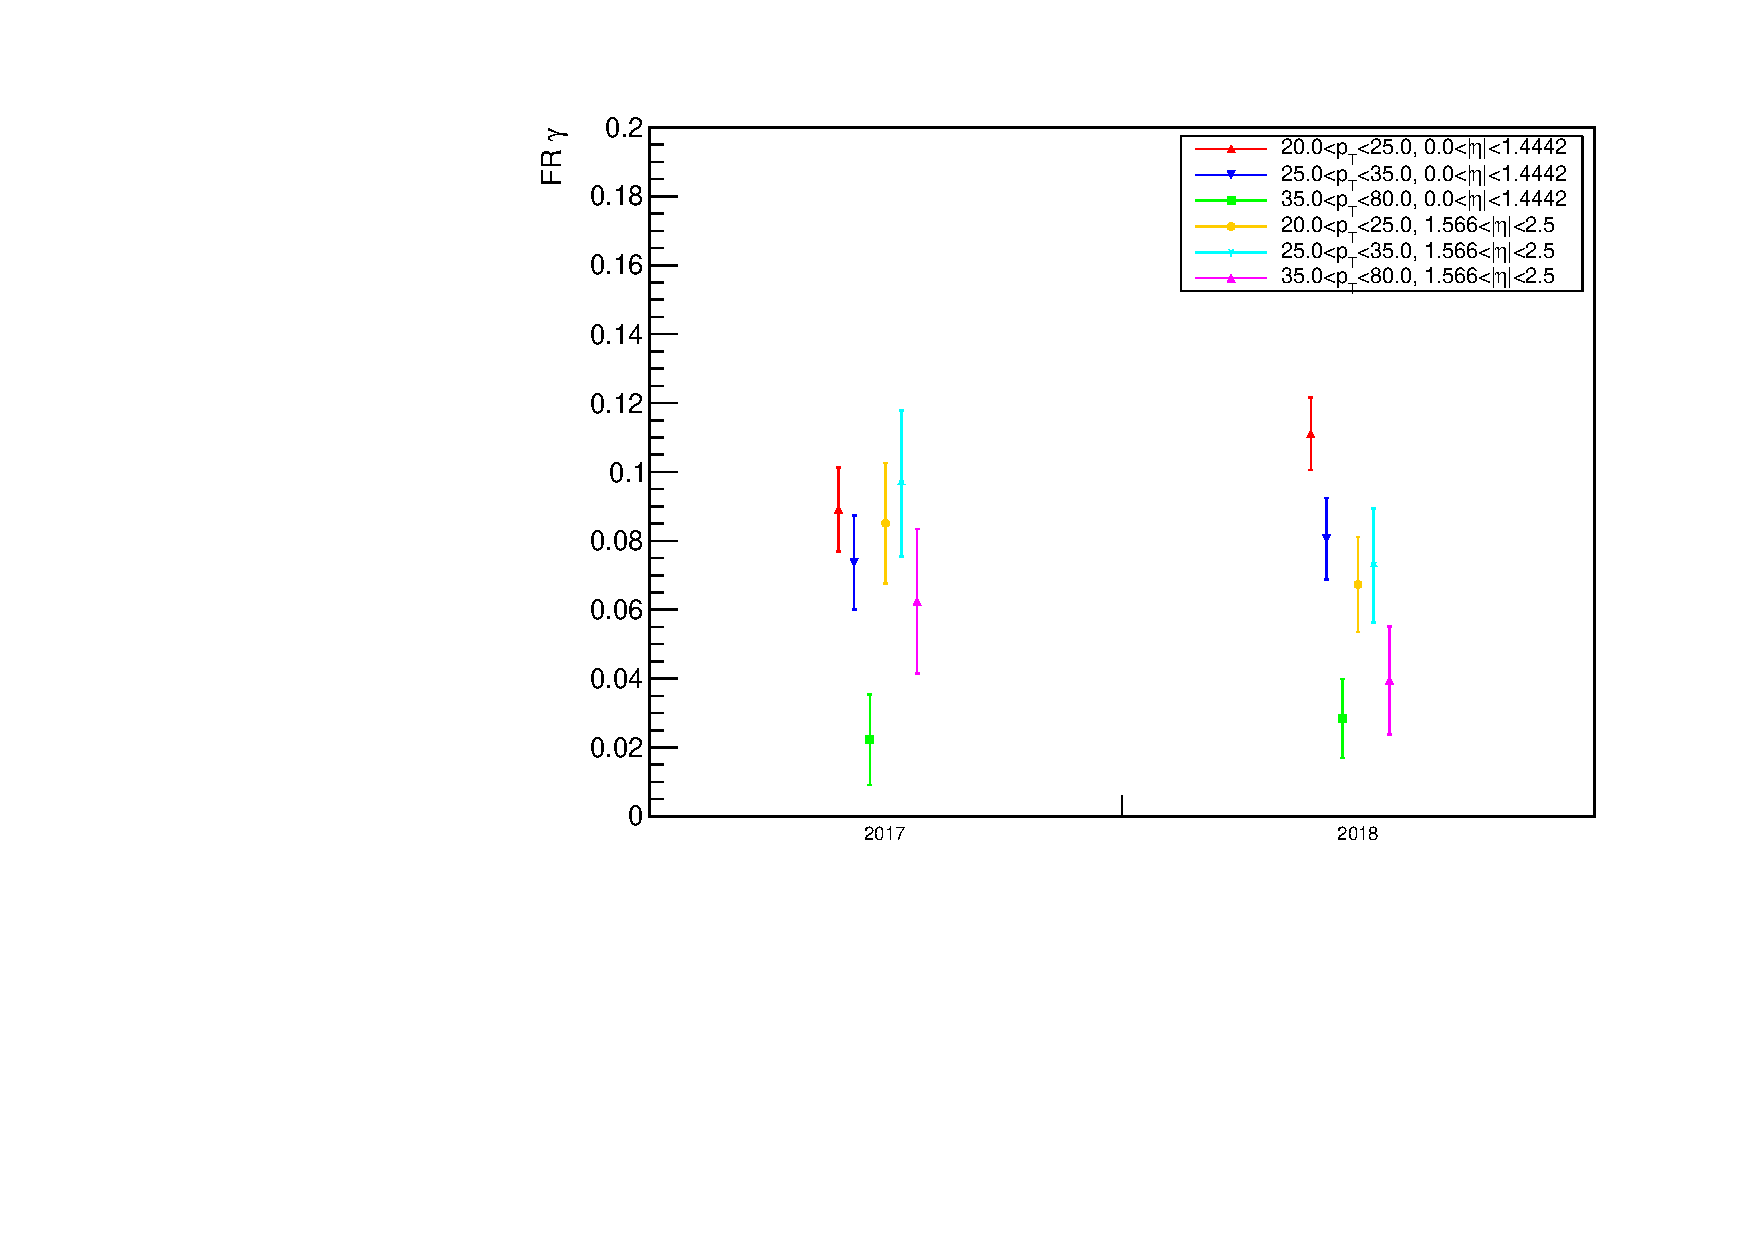
\includegraphics[width=.5\textwidth]{Figures/FR_VLtoL_pt-aeta_data-ZGToLLG_time.pdf}
\caption{Photon non-prompt rate in different data-taking periods.}
\label{fig:phFR_time}
\end{figure}

\subsubsection{Photon fake rate application}
The Fake Rate is then applied to events in the CR4P\_1F, CR3P\_1F and CR2P\_1F regions to estimate the non-prompt contribution in SR4P\_1P, SR3P\_1P, SR3P\_1P respectively.
Each event in this region is reweighed by the transfer factor $TF^\gamma(p_T, \eta) = \frac{f^\gamma}{1-f^\gamma}$, where $f^\gamma$ is the Fake Rate estimated in the measurement region.

\begin{equation}
  \begin{split}
    \label{eq:fakeRate_explanation_part1}
    N^{bkg}_{4P\_1P} &= \sum f_i N^{bkg}
    \\
    N^{bkg}_{4P\_1F} &= \sum ( 1-f_i ) N^{bkg}
  \end{split}
\end{equation}
where $N^{bkg}$ is the total number of events that have a fake photon, regardless of the region they are classified into.
From this it follows that the number of background events in the signal region is:
\begin{equation}
  \label{eq:fakeRate_explanation_part2}
  N^{bkg}_{4P\_1P} = \sum \frac{f_i}{1-f_i} N_{4P\_1F}
\end{equation}

\paragraph{Usage of the MVA based ID\\}
Additionally, kinematic photons that pass the MVA-based working points wp90 and wp80 are also considered,
given the improved performance of the MVA ID over the cut-based one.
The drawback is that this does not allow a data-driven estimation of the \nonprompt background,
due to the limited size of the application region defined by requiring a photon that passes the wp90 but fails the wp80.

Unlike a cut-based selection, it is not possible to invert only part of the MVA based ID.
The only way to derive a looser working point is to redo the optimisation of the raw MVA score,
and then study the efficiency of such selection in data and simulation to derive scale factors.
Both of these studies are outside the scope of this analysis.

Another possibility is to measure a fake rate between the kinematic selection and the looser MVA working point, \texttt{wp90}.
However, the former is too loose and the selected fakes have signatures that are very different from those of prompt photons.
This would make the assumption that the transfer factor is the same in the measurement and application regions quite unstable.

\todo{Add plots (e.g. Data/MC of CR3P1F/CR2P2F o SR4P blinded) of the number of events in wp90, wp80.}

Therefore, the results obtained using the MVA ID are derived without the data-driven estimate of fake photons.
In this case, the MC prediction of backgrounds which contain \nonprompt or misidentified photons is used.

\subsection{Final State Radiation}
\todo{TODO after discussion on ZZ and ZZgamma.}
